\chapter{Material und Methoden}
\label{chap:material}
\section{Business Understanding}
\label{sec:BU}
In der ersten Phase des CRISP-DM Modells geht es um das gezielte Verstehen der gegebenen Problemstellung. In der konkret vorliegenden Aufgabenstellung, soll eine Entscheidung getroffen werden, ob einem Kunden nach seinem Einkauf auf der Plattform des Online-Händlers ein Gutschein in Höhe von 5 \euro{} zugesendet werden soll oder nicht.\\
 
Die Entscheidung soll automatisiert durch einen binären Klassifikator getroffen werden. Der Klassifikationsalgorithmus soll Kunden in zwei Gruppen einteilen. Die erste Klasse beinhalten Kunden, welche keine Folgebestellung abgegeben haben. Die zweite Klasse umfasst dagegen alle Wiederkäufer. Die Einteilung in die beiden Klassen findet auf Basis eines gegeben Zeitrahmens von 90 Tagen nach der Erstbestellung statt.  Käufer, welche erst nach Überschreitung dieses Zeitraums einen Kauf tätigen, werden nicht als Wiederkäufer betrachtet.\\

Ziel ist es mittels Vergangenheitsdaten über die Eigenschaften von Kunden und ihren Bestelldetails ein Modell zu erstellen, welches Regeln über Klassenzugehörigkeiten ableitet. Damit sollen Kunden durch einen Algorithmus automatisiert als Wiederkäufer (Klasse 1) und keine Wiederkäufer (Klasse 0) eingeordnet werden. Ziel ist eine intelligente Vergabe der Gutscheine, womit eine Umsatzmaximierung erreicht werden soll. Für die Evaluation dieses Zieles, liegt folgende  Kostenmatrix vor:\\

\begin{table}[h]
\centering
\small
\begin{tabular}{c r|c|c|}
            & & \multicolumn{2}{c|}{Vorhergesagt}             \\
            &	&kein Wiederkäufer(0)   &Wiederkäufer(1)            \\ \hline
            \multirow{2}*{Tatsächlich} &kein Wiederkäufer(0)&1.5   &0               \\
            &Wiederkäufer(1)&-5   &0              \\ \hline
      \end{tabular}
      %\caption{Kostenmatrix}
\end{table}

Nach dieser Kostenmatrix entsteht ein Verlust in Höhe von 5 \euro{}, wenn einem tatsächlichen Wiederkäufer ein Gutschein zugesendet wird, weil er als Nicht-Wiederkäufer klassifiziert worden ist. Wird einem tatsächlichen Nicht-Wiederkäufer ein Gutschein zugesendet, weil er als ebendieser klassifiziert wird, so erhöht das den Gewinn des Online-Händlers um 1,50 \euro{}.\\

Nach dieser Kostenmatrix hat eine Fehlklassifikation eines tatsächlichen Wiederkäufers als Nicht-Wiederkäufer die größten Auswirkungen. Ziel sollte es demnach sein, in erster Priorität die Wiederkäufer korrekt zuzuordnen und in zweiter Priorität die Nicht-Wiederkäufer zu identifizieren. Im nächsten Schritt werden die vorhandenen Daten genauer untersucht.\\


\pagebreak
\section{Data Understanding}
\label{sec:datensatz}
Beim Data Understanding wird versucht die Daten möglichst gut zu verstehen, um anschließend geeignete Werkzeuge der Datenbehandlung auswählen zu können. Dabei werden geeignete Methoden der deskriptiven Statistik genutzt, um aussagekräftige Kennzahlen und Visualisierungen zu erstellen. Es wird der Grundstein für die Vorverarbeitung der Daten gelegt. Die Evaluation, ob ein Merkmal zur Klassifikationsgüte beitragen kann, basiert schließlich auf dem Verständnis der Daten. Des Weiteren können in dieser Phase Ideen für die Erstellung neuer Merkmale generiert werden.\\

Damit ein Lernalgorithmus gute Ergebnisse liefern kann, sind in der Regel viele Trainingsdaten nötig. Der gegebene Trainingsdatensatz besteht aus 10470 Einträgen mit 38 Merkmalen. Eines davon ist die Zielvariable „target90. Diese codiert in binärer Darstellung, ob ein Kunde innerhalb von 90 Tagen wiedergekauft hat. Die Zielvariable soll anhand eines überwachten Lernverfahrens für die Testdaten vorhergesagt werden. Anhand der Größe der Trainingsdaten, kann von einer angemessenen Stichprobengröße ausgegangen werden.\\

Nichtsdestotrotz ist ein großer Trainingsdatensatz keine Garantie für gute Ergebnisse. Das ist genau dann der Fall, wenn die Merkmale nicht repräsentativ für eine möglichst überschneidungsfreie Zuordnung der Klassen sind. Es gilt daher auch im Bereich des Data Understandings und der anschließenden Phase der Vorverarbeitung (Data Preparation) zu ermitteln, durch welche Modifikation sich die Daten am besten für die Modellbildung eignen. Das bedeutet, inwiefern sich transformierte Merkmale zu einer Verallgemeinerung und infolgedessen zum Erlernen von Regeln bezüglich der Zielvariable eignen. Dabei muss zusätzlich überprüft werden, welche Daten sich qualitativ eignen. Der Umgang mit fehlenden und falschen Werten ist nötig. Zudem müssen Ausreißer behandelt werden, um Rauschen in den Daten zu vermindern.\\

Der gegebene Testdatensatz besteht aus 2521 Einträge. Ohne Vorverarbeitung der Daten ergibt sich ein Aufteilungsverhältnis von ungefähr 80:20. Das heißt, dass auf 80 \%  der Daten ein Modell trainiert wird, welches auf 20 \% der Daten getestet wird. Diese Aufteilung ist durch die Aufgabenstellung fest vorgegeben. Der Testdatensatz wird in den folgenden Phasen prinzipiell nicht genauer untersucht, sodass sich das reale Szenario ergibt, dass die neu zu klassifizierenden Daten mit ihren Klassenlabels unbekannt sind und eine Überanpassung an die Datensätze vermieden werden soll.\\

Dennoch kann sich eine Veränderung des Verhältnisses zwischen den beiden Datensätzen im weiteren Verlauf ergeben. Das liegt daran, dass die Trainingsdaten bestimmten Transformationen unterliegen. Beispielsweise könnten Einträge, aufgrund fehlender Werte, gelöscht werden. Zum anderen könnten die Trainingsdaten durch Resampling-Methoden artifiziell vergrößert oder verkleinert werden. Diese Veränderungen werden genauer in der Data Preparation Phase erläutert.\\ 

Im Folgenden wird damit begonnen die einzelnen Merkmale auf Basis der Trainingsdaten genauer zu beschreiben und mit geeigneten statistischen Hilfsmitteln und Visualisierungen zu untersuchen.
\pagebreak
\begin{table}[]
\subsection{Der Datensatz}
\centering
%\begin{tabular}{l r}
\begin{tabular*}{\textwidth}{c @{\extracolsep{\fill}} cc}
\toprule
\textbf{Merkmal} & \textbf{Beschreibung} \\
\midrule
 customernumber & individuelle Kundennummer\\
 \hline
 date & Datum der ersten Bestellung\\
 \hline
 salutation & Anrede des Kunden bzw. Firmenkunde\\
 \hline
 title & Titel vorhanden oder nicht\\
 \hline
 domain & Domain des Email Providers\\
 \hline
 datecreated & Datum der Accounterstellung\\
 \hline
 newsletter & wurde der Newsletter abboniert\\
 \hline
 model & nicht spezifiziert (Werte: 1,2,3)\\
 \hline
 paymenttype & gewählter Zahlungstyp\\
 \hline
 deliverytype & Versandart\\
 \hline
 invoicepostcode & Rechnungsadresse\\
 \hline
 delivpostcode & Lieferadresse\\
 \hline
 voucher & wurde ein Gutschein eingelöst\\
 \hline
 advertising & Werbecode\\
 \hline
 case & Wert der bestellten Produkte\\
 \hline
 numberitems & Anzahl der bestellten Artikel\\
 \hline
 gift & wurde die Geschenkoption verwendet\\
 \hline
 entry & Zugang zum Shop durch einen Partner oder nicht\\
 \hline
 points & wurden Punkte eingelöst\\
 \hline
 shippingcosts & sind Versandkosten angefallen\\
 \hline
 deliverydatepromised & versprochenes Lieferdatum\\
 \hline
 deliverydatepromised & tatsächliches Lieferdatum\\
 \hline
 weight & Gewicht der Bestellung\\
 \hline
 remi & Anzahl zurückgesendeter Artikel\\
 \hline
 cancel & Anzahl stornierter Artikel\\
 \hline
 used & Anzahl gebrauchter Artikel\\
 \hline
 w0 & Anzahl bestellter gebundener Bücher\\
 \hline
 w1 & Anzahl bestellter Taschenbücher\\
 \hline
 w2 & Anzahl bestellter Schulbücher\\
 \hline
 w3 & Anzahl bestellter eBooks\\
 \hline
 w4 & Anzahl bestellter Hörbücher\\
 \hline
 w5 & Anzahl heruntergeladener Hörbücher\\
 \hline
 w6 & Anzahl bestellter Filme\\
 \hline
 w7 & Anzahl bestellter Musikartikel\\
 \hline
 w8 & Anzahl bestellter Hardwareartikel\\
 \hline
 w9 & Anzahl bestellter importierter Artikel\\
 \hline
 w10 & Anzahl sonstige bestellte Artikel\\
 \hline
 \textbf{target90} & Zielvariable: Folgebestellung innerhalb von 90 Tagen oder nicht\\
\bottomrule
\end{tabular*}
\label{table: Features}
\caption{Übersicht aller Merkmale}
\end{table}
\FloatBarrier
\pagebreak
\subsection{Die Zielvariable}

Die Zielvariable target90 gibt an, ob ein Kunde innerhalb von 90 Tagen erneut eine Bestellung beim Online-Händler getätigt hat oder nicht. Es handelt sich um eine nominalskalierte Variable, welche als Ganzzahl codiert worden ist. Das Klassenlabel ist in Trainings- und Testdatensatz für alle Einträge angegeben. Deswegen handelt es sich hierbei um überwachtes Lernen. Dadurch, dass ausschließlich zwei Ausprägungen möglich sind, bezeichnet man die Aufgabenstellung als binäre Klassifikation.\\

In Abbildung \ref{fig:classDist} ist die Verteilung der Zielvariable für Trainings- und Testdaten dargestellt. Es wird deutlich, dass in beiden Datensätzen eine ähnliche Verteilung vorliegt. Rund 80 \% der Einträge nehmen die Ausprägung 0 an. Das heißt, dass 80 \% der Kunden nach der Erstbestellung nicht innerhalb von 90 Tagen erneut bestellen. Dagegen sind 20 \% der Kunden als Wiederkäufer etikettiert. Diese Verteilung zeigt die Unbalanciertheit der beiden Klassen.\\

Die fehlende Gleichverteilung kann im Zuge der Modellbildung und Klassifikation zu falschen Ergebnissen führen. Das begründet sich darin, dass die meisten Algorithmen implizit eine Gleichverteilung der Klassen annehmen. Es gibt deutlich weniger Trainingsbeispiele, um die Eigenschaften der unterrepräsentierten Klasse zu erlernen. Das kann zu Klassifikatoren führen, welche lediglich die überrepräsentierte Klasse vorhersagen. Diese Beobachtung führt dazu, dass im späteren Verlauf des Modellbildungsprozesses Resampling-Strategien angewendet werden.

\begin{figure}[!htbp]
\begin{center}
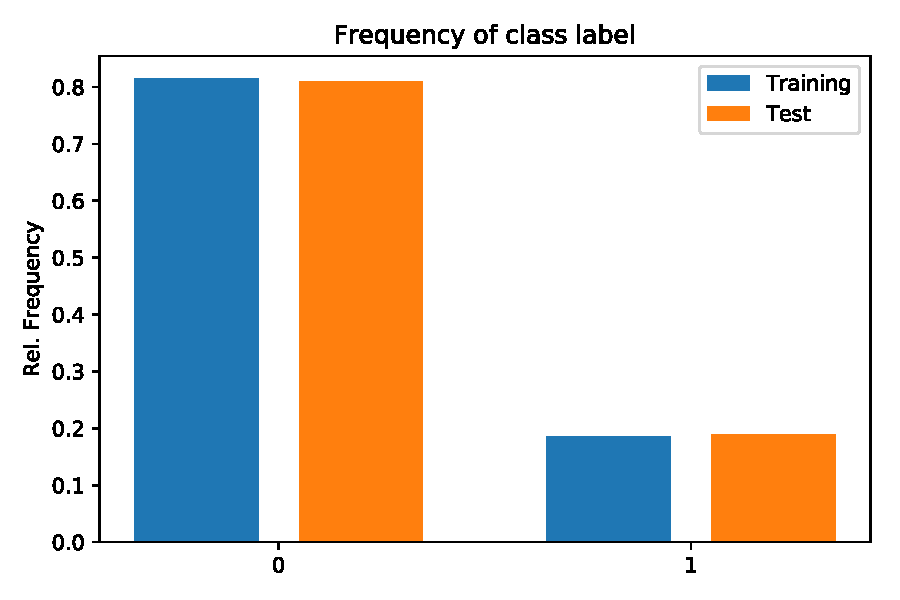
\includegraphics[scale=0.5]{pdf/classDist.pdf}
\end{center}
\caption{Klassenverteilung in Trainings- und Testdaten}
\label{fig:classDist}
\end{figure}
\FloatBarrier
\pagebreak

\subsection{Kategoriale Merkmale}

Einschließlich der Zielvariable enthält der Datensatz 18 kategoriale Merkmale. Bis auf das ordinalskalierte Merkmal case, welches den Wert der bestellten Güte durch Kategorien ausdrückt, sind alle anderen Merkmale nominalskaliert. Die meisten dieser Merkmale sind als Zahl repräsentiert. Es ist dabei zu berücksichtigen, dass sich nominalskalierte Merkmale in keine Reihenfolge bringen lassen, welche Aussagen der Form „besser oder schlechter als“ zulassen. Als Kennzahlen sind deshalb nur solche gestattet, welche die Häufigkeiten berücksichtigen. Ein Maß ist der Modus. Dieser gibt die Ausprägung mit der größten relativen bzw. absoluten Häufigkeit an. Aufgrund der mangelnden Kennzahlen, werden die relevanten kategorialen Merkmale in Abbildung \ref{fig:distC2} bezüglich ihrer Häufigkeitsverteilung unter Berücksichtigung der beiden Klassen visualisiert.\\

Auf der Abszisse werden sämtliche Ausprägungen des Merkmals abgetragen. Die Ordinate gibt die absolute Häufigkeit der Ausprägungen an. Generell ist sehr auffällig, dass sich die Klassenverteilung von 80:20 deutlich in den kategorialen Merkmalen widerspiegelt. Diese Eigenschaft bedeutet eine geringe Abhängikeit zwischen Merkmal und Klasse und ist ungünstig bei Klassifikationsaufgaben. Die Begründung dafür ist, dass die unterschiedlichen Ausprägungen nicht gut zur Separation der Klassen beitragen.\\ 

Visuell verspricht das Merkmal newsletter tendenziell bessere Ergebnisse. Die Klassenverteilung unter der Bedingung Newsletter abonniert (1) zeigt eine visuell geschätzte Aufteilung von 60:40 der Klassen. Das führt zu der Interpretation, dass Kunden, welche einen Newsletter abonniert haben, eher zum Wiederkauf neigen. Ebenso vielversprechend wirkt das Merkmal Warenwert (case). Dieses zeigt, dass die Erstbestellungen mit hohem Warenwert einen relativ höheren Anteil an Wiederkäufern enthalten als der gesamte Trainingsdatensatz. Die gefundenen Auffälligkeiten werden im Teil der Modellevaluation mittels einer Backward Feature Selection überprüft.\\
 
Negativbeispiele für die Separierung der beiden Klassen sind die Merkmale Geschenkoption gewählt (gift), Punkte eingelöst (points) und Titel angegeben (title). Diese Merkmale besitzen teilweise nur eine Ausprägung, bzw. sehr geringe absolute Häufigkeiten bezüglich der zweiten Ausprägung. Damit sind diese Features überhaupt nicht dazu geeignet die Klassifikationsgüte zu verbessern. Diese Beobachtungen bilden die Grundlage für das Löschen dieser Merkmale im Teil Data Preparation. 


\begin{figure}[!htbp]
\begin{center}
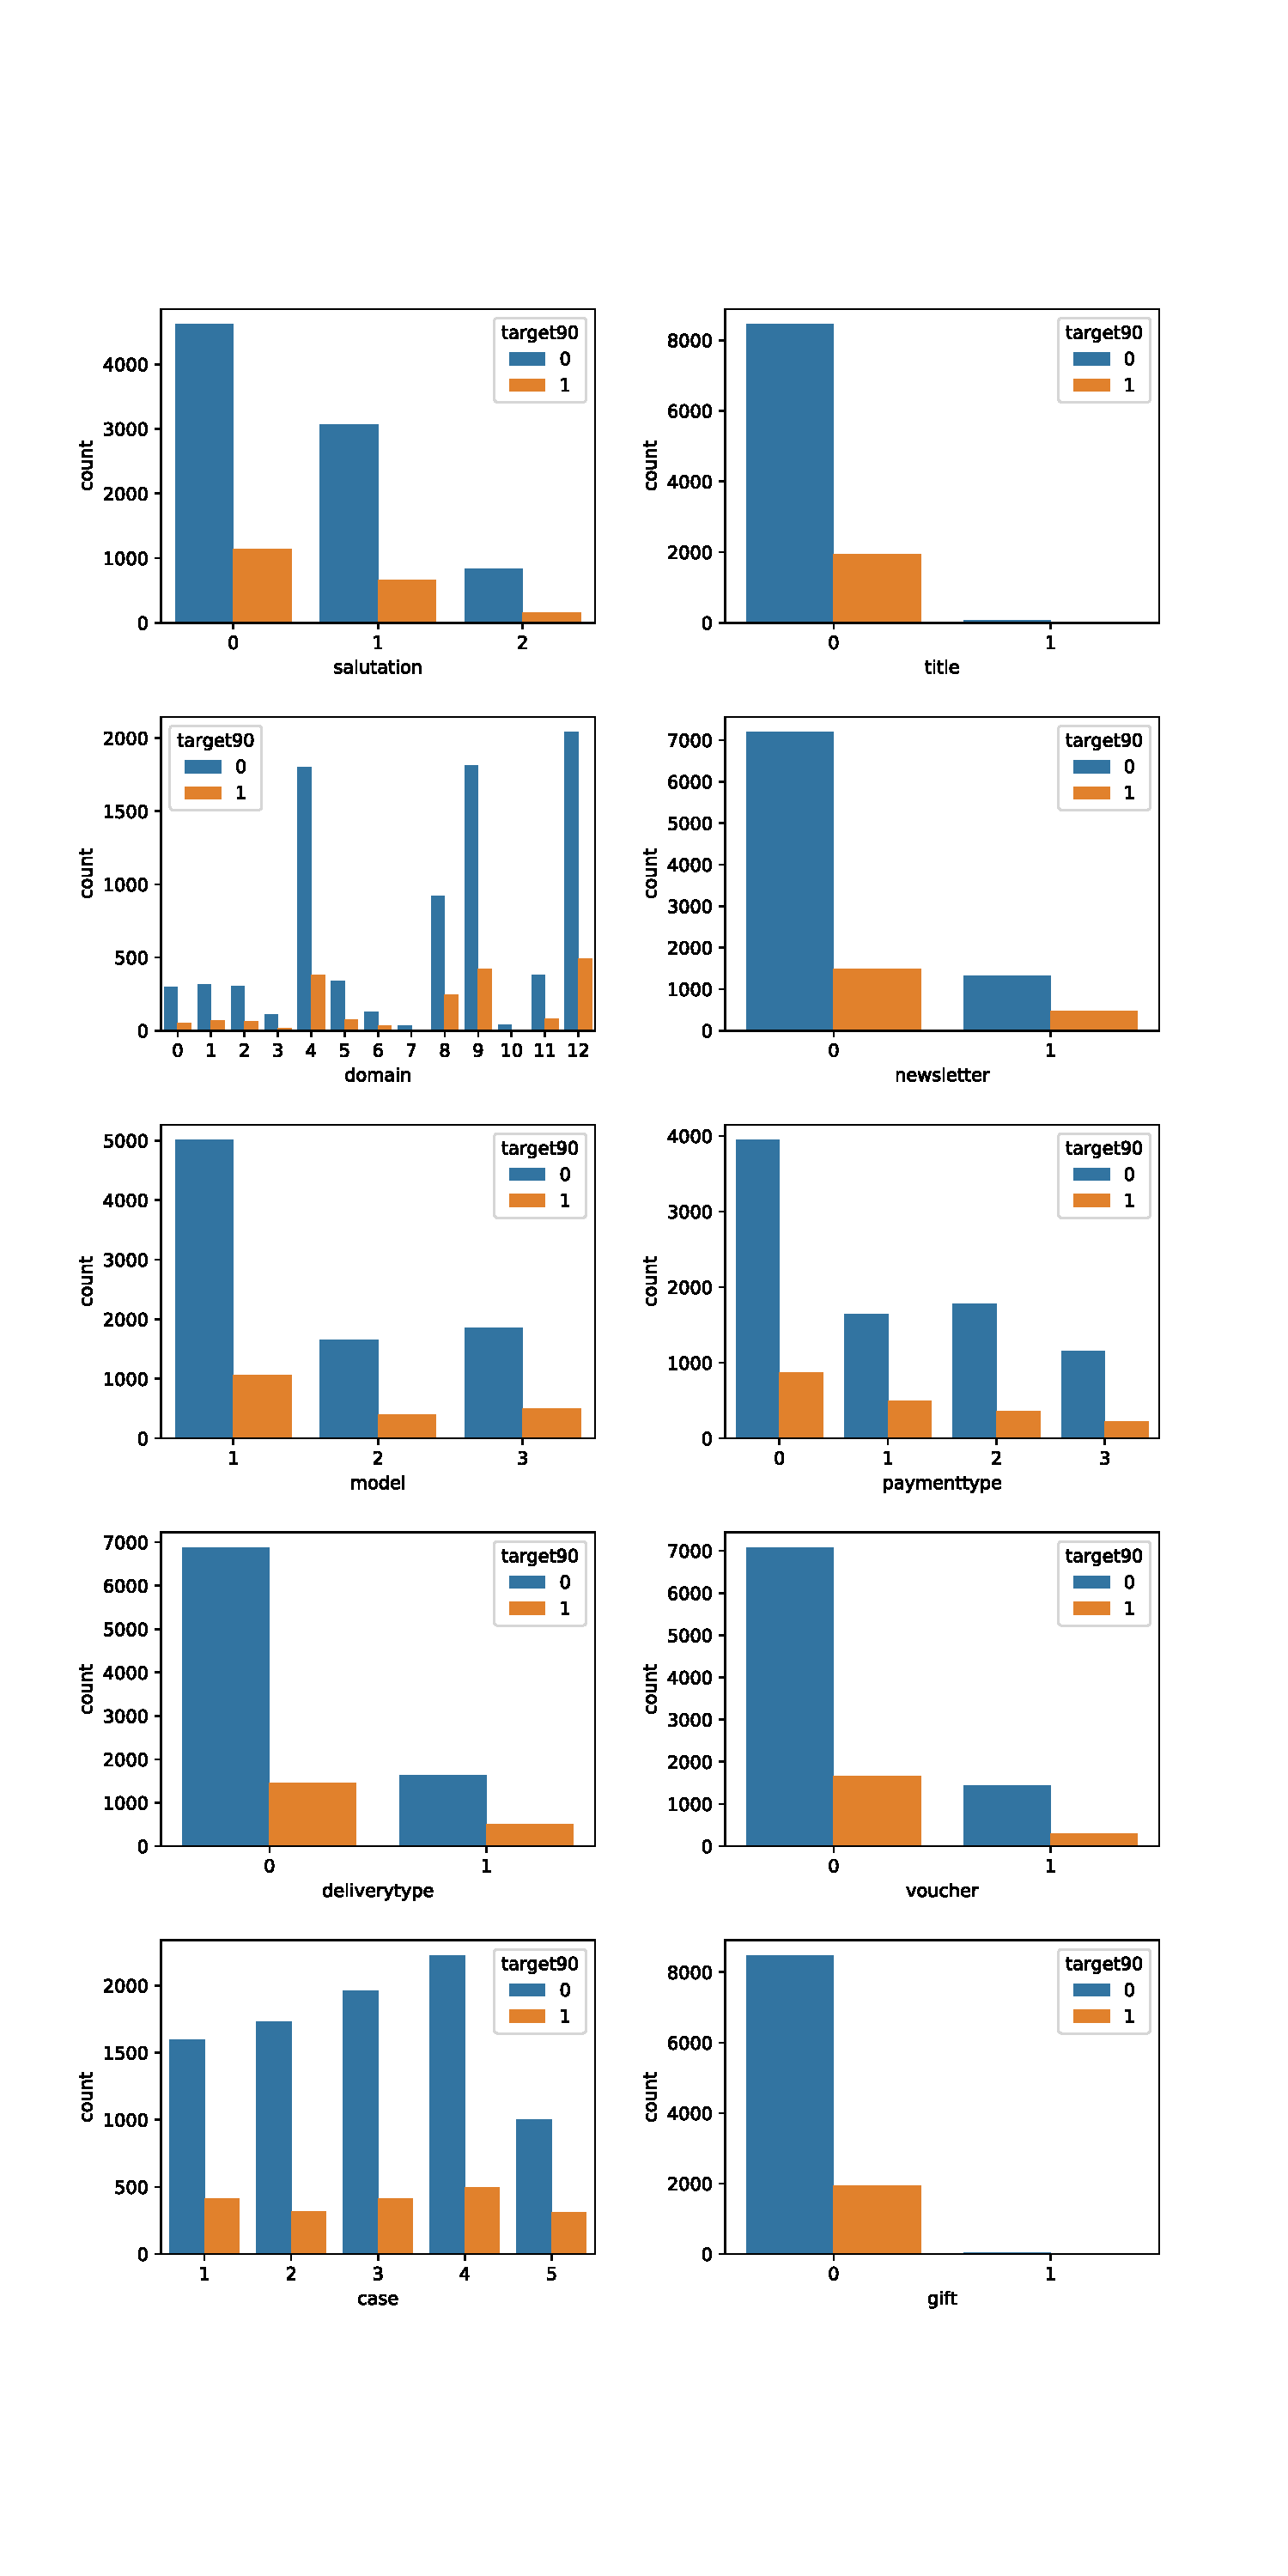
\includegraphics[scale=0.5]{pdf/distCategorical.pdf}
\end{center}
\label{fig:distC}
\end{figure}
\begin{figure}[!t]
\begin{center}
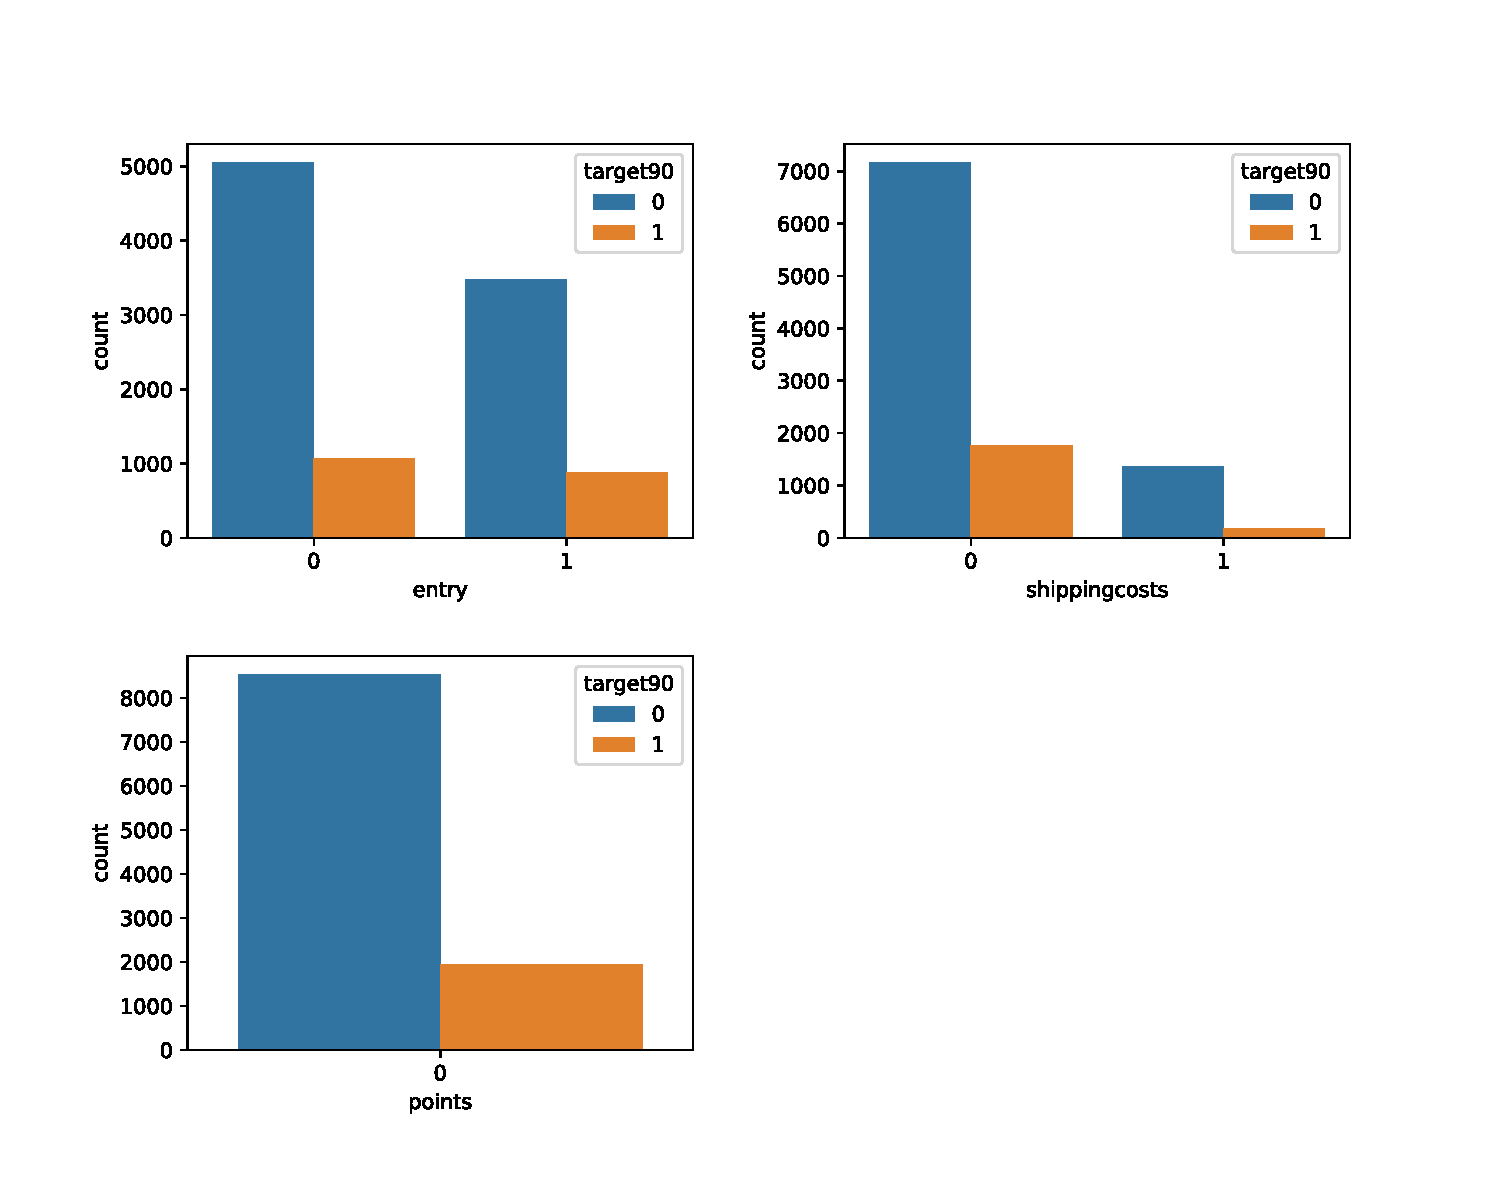
\includegraphics[scale=0.5]{pdf/distCategorical2.pdf}
\end{center}
\caption{Verteilung nominal- und ordinalskalierte Merkmale}
\label{fig:distC2}
\end{figure}
\FloatBarrier
\pagebreak

\subsection{Numerische Merkmale}
Der Datensatz enthält 20 kardinalskalierte Merkmale. Im Gegensatz zu den kategorischen Merkmalen lassen sich für diese Merkmale Kennzahlen wie Mittelwert, Standardabweichung, Median und Quantile berechnen. Bevor geeignete Visualisierungen erstellt und Kennzahlen berechnet werden, sind diese Merkmale auf fehlende Werte und Ausreißer zu prüfen. Diese können dazu führen, dass die Berechnungen nicht funktionieren bzw. verzerrt werden. Zudem können die meisten Algorithmen des maschinellen Lernens nicht mit fehlenden Werten umgehen.\\

\textbf{Fehlende Werte:}\\

Beim Umgang mit fehlenden Werten ist zu entscheiden, wie mit diesen umgegangen werden soll. Dabei gibt es unterschiedliche Wege diese zu behandeln. Fehlende Werte können durch Kennzahlen wie zum Beispiel Mittelwert und Median ersetzt werden. Bei einer genügenden Anzahl an Trainingsdaten, kann sich dafür entschieden werden entsprechende Datenpunkte komplett aus dem Datensatz zu löschen. Hierbei muss beachtet werden, wie oft fehlende Werte bei den verschiedenen Merkmalen vorkommen. Im schlimmsten Fall führt das Löschen der Datenpunkte zu einer drastischen Reduzierung der Trainingsdaten. Deshalb kann stattdessen das Löschen eines kompletten Merkmals in Frage kommen.\\ 

Zur Zielstellung dieser Arbeit gehört die Bildung von eindeutig definierten Schritten der Datenvorverarbeitung. Diese werden in Funktionen festgehalten und können somit unmittelbar auf die Trainings- und Testdaten angewendet werden. Dies stellt eine konsistente Transformation der beiden Datensätze sicher. Ein Löschen von Datenpunkten würde deshalb auch zu einer Reduzierung des Testdatensatzes führen. Daher wird versucht, fehlende Werte möglichst zu ersetzen.\\ 

Ist der Anteil fehlender Werte groß, wird stattdessen das komplette Merkmal gelöscht. Ein weiteres Argument für das Löschen von Merkmalen ist die hohe Anzahl der Merkmale. Des Weiteren kann im Zuge der Evaluation eines Klassifikators das Merkmal wieder in die Merkmalsmatrix aufgenommen werden und fehlende Werte mit einer Auffüllungsstrategie behandelt werden. Anschließend kann bewertet werden, ob dieses Merkmal aufgrund einer Performancesteigerung des Klassifikators doch berücksichtigt werden sollte. Dieses Vorgehen zeigt den Charakter des CRISP-DM Modells. Es handelt sich um einen rollierenden Prozess, in welchem immer wieder auf die Vorgängerphasen zurückgeschaltet werden kann, um insgesamt die Ergebnisqualität zu erhöhen.\\

Bei der Untersuchung der numerischen Features hat sich herausgestellt, dass nur das versprochene Lieferdatum (deliverydatereal) fehlende Werte enthält. Diese treten jedoch immer in Kombination mit der Bestellung digitaler Artikel auf. Im Kontext des Business Understandings kann deshalb davon ausgegangen werden, dass diese Produkte nicht geliefert werden und direkt heruntergeladen werden können. Daher wird das versprochene Lieferdatum für diese Werte eingesetzt. Beim späteren Feature Engineering wird das Merkmal Lieferverzug erstellt. Bei downloadfähigen Produkten entsteht deshalb kein Lieferverzug.\\ 

\textbf{Ausreißer}\\

In diesem Abschnitt wird diskutiert, wie Ausreißer im Datensatz behandelt werden. Prinzipiell gibt es verschiedene Strategien, um Ausreißer zu behandeln: Man kann die Werte durch Kennzahlen aus der deskriptiven Statistik ersetzen. Häufig bevorzugte Werte sind der Median oder das arithmetischen Mittel. Beim arithmetischen Mittel ist darauf zu achten, dass dieses gerade anfällig für Ausreißer ist. Diese Strategien kann man je nach vorhandenem Verständnis der Daten und der Zielsetzung der Aufgabenstellung individuell für jedes Merkmal anpassen. Diese Ersetzungstrategie kann multivariat durchgeführt werden. Das heißt, dass  die Kennzahl nicht von allen Beobachtungen des Merkmals berechnet wird, sondern in Abhängigkeit von den Merkmalsausprägungen anderer Merkmale.\\

Darüber hinaus können bei genügend zeitlichen Ressourcen Ausreißer auf Validität geprüft werden. Bei einem Ausreißer kann nicht sofort auf einen falschen Wert geschlossen werden. Denn ein Ausreißer kann auch die Streuung der Merkmalsausprägungen repräsentieren. Um den originalen Trainingsdatensatz nicht zu modifizieren, wird eine Kopie der Trainingsdaten erstellt, in welcher die numerischen Features extrahiert worden sind. Damit können zunächst Transformationen getestet werden. Bei der Behandlung von Ausreißern steht, wie bei der Behandlung von fehlenden Werten, die Reproduzierbarkeit und das Anwenden von generischen Funktionen im Vordergrund. Damit wird sichergestellt das entsprechende Transformationen sowohl auf Trainings– als auch Testdaten angewendet werden kann. Daher wird auf die individuelle Betrachtung von Ausreißern verzichtet. Stattdessen werden die numerischen Merkmale zunächst durch Boxplots in Abbildung \ref{fig:boxplot} visuell überprüft und anschließend wird in Tabelle \ref{table: outlier} der Ausreißeranteil dargestellt.\\

In Abbildung \ref{fig:boxplot} sind bis auf die Datumswerte, welche extra behandelt werden, alle kardinalskalierten Merkmale mittels Boxplot visualisiert worden. Sehr auffällig ist, dass bei fast allen Merkmalen die Box fehlt. Die Box besteht aus allen Werten, welche zwischen dem ersten und dritten Quartil liegen. Bis auf die Anzahl der bestellten Artikel, das Gewicht und die Anzahl bestellter gebundener Bücher, haben alle anderen Merkmale einen Median von 0. Durch den fehlenden Interquartilsabstand sind deshalb alle von 0 verschiedenen Werte als Ausreißer durch einen Punkt gekennzeichnet. Ausreißer sind nach dieser Definition alle Werte die größer oder kleiner als der 1,5-fache Interquartilsabstand sind. Dadurch, dass keine negativen Ausprägungen der Merkmale möglich sind, gibt es nur Ausreißer in eine Richtung.\\

\FloatBarrier
\begin{figure}[!htbp]
\begin{center}
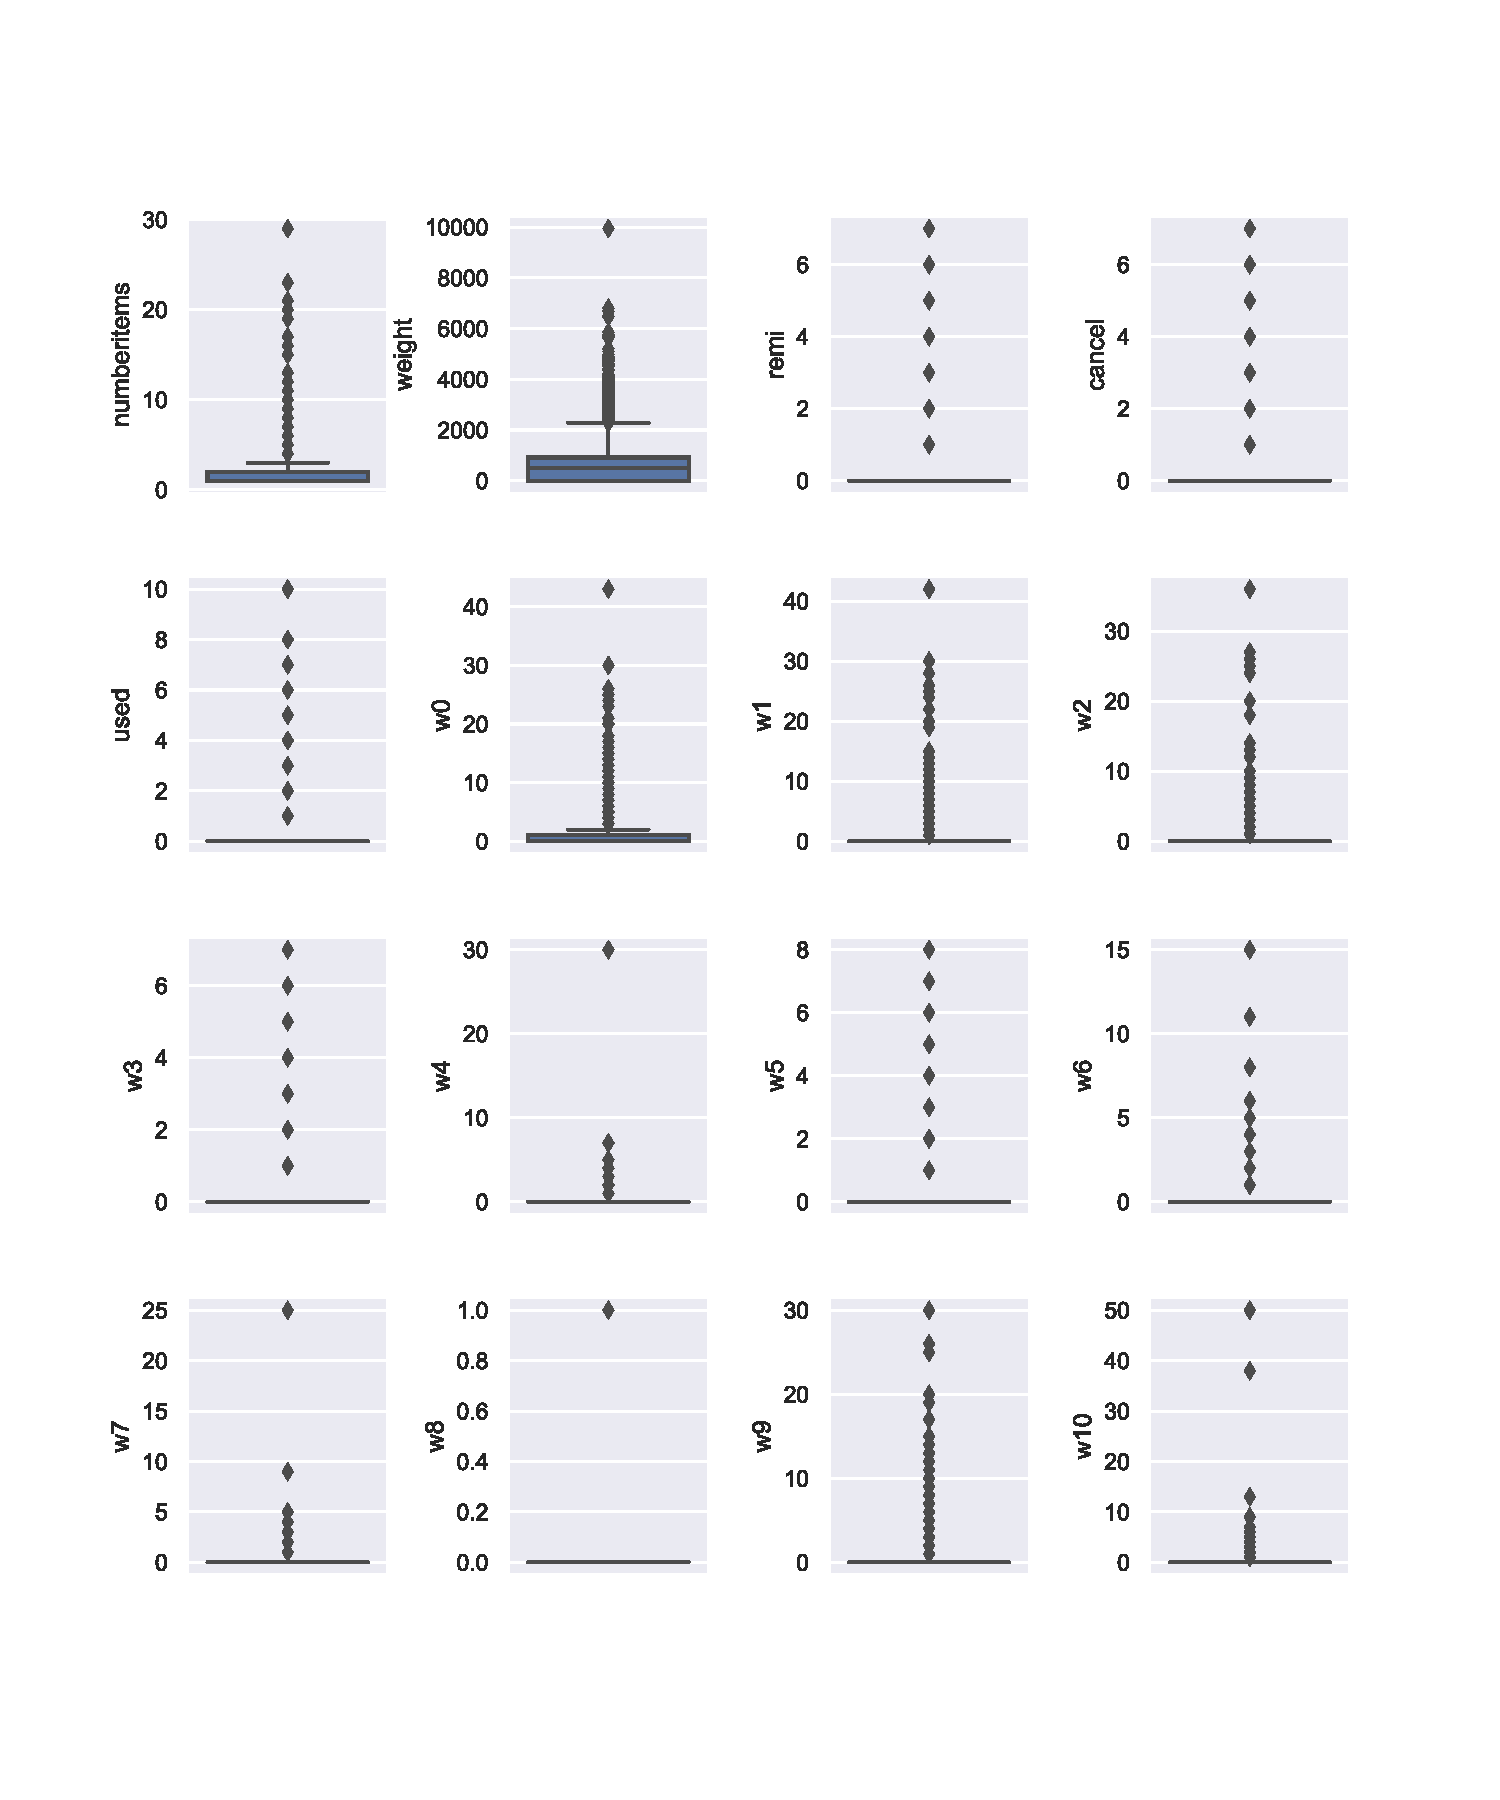
\includegraphics[scale=0.6]{pdf/boxplot.pdf}
\end{center}
\caption{Boxplot der numerischen Merkmale}
\label{fig:boxplot}
\end{figure}
\FloatBarrier

In Tabelle \ref{table: outlier} ist zu jedem Merkmal Median, Interquartilsabstand, Mittelwert und Standardabweichung berechnet worden. Des Weiteren wird der Anteil der Ausreißer quantifiziert. Wie bereits visuell entdeckt, existiert bei fast allen Merkmalen kein Interquartilsabstand. Deshalb sind alle von 0 verschiedenen Werten automatisch größer gleich dem 1.5 fachen Interquartilsabstand und nach dieser Definition ein Ausreißer. Unter allen Merkmalen, welche eine Anzahl bestellter Artikel angeben, überschreiten kaum welche die Anzahl von 40. Im Kontext des Business Understandings ist diese Anzahl an bestellten Artikeln nicht unrealistisch, da der Online-Händler schließlich auch zahlreiche Firmenkunden hat. Es wird deshalb nach dieser Analyse der Beschluss gefasst, dass zunächst keine Ausreißer gelöscht werden und alle Merkmalsausprägungen als valide angenommen werden.\\

\FloatBarrier
\begin{table}[!htbp]
\centering
%\begin{tabular}{c r l c c c}
\begin{tabular*}{\textwidth}{c @{\extracolsep{\fill}} lllllll}
\toprule
\textbf{Merkmal} & \textbf{Median} & \textbf{IQR}  & \textbf{Ausreißer} & \textbf{Mean} & \textbf{STD}\\
\midrule
numberitems & 1.0 & 1.00 & 12.70 \% & 2.00 & 1.64 \\
weight & 496.0 & 914.00 & 2.96 \% & 634.97 & 691.51\\
remi & 0.0 & 0.00 & 100.00 \% & 0.06 & 0.37\\
cancel & 0.0 & 0.00 & 100.00 \% & 0.06 & 0.30 \\
used & 0.0 & 0.00 & 100.00 \% & 0.07 & 0.44\\
w0 & 1.0 & 1.00 & 7.98 \% & 0.90 & 1.47\\
w1 & 0.0 & 0.00 & 100.00 \% & 0.38 & 1.31\\
w2 & 0.0 & 0.00 & 100.00 \% & 0.28 & 1.20\\
w3 & 0.0 & 0.00 & 100.00 \% & 0.02 & 0.19\\
w4 & 0.0 & 0.00 & 100.00 \% & 0.04 & 0.41\\
w5 & 0.0 & 0.00 & 100.00 \% & 0.17 & 0.53\\
w6 & 0.0 & 0.00 & 100.00 \% & 0.03 & 0.29\\
w7 & 0.0 & 0.00 & 100.00 \% & 0.02 & 0.33\\
w8 & 0.0 & 0.00 & 100.00 \% & 0.00 & 0.01\\
w9 & 0.0 & 0.00 & 100.00 \% & 0.18 & 0.91\\
w10 & 0.0 & 0.00 & 100.00 \% & 0.09 & 0.75\\
\bottomrule
\end{tabular*}
\caption{Ausreißer numerische Merkmale}
\label{table: outlier}
\end{table}
\FloatBarrier

\textbf{Korrelationsanalyse}\\

Bei der Korrelationsanalyse ist der Korrelationskoeffizient nach Pearson zwischen den numerischen Merkmalen berechnet worden. Bei der Analyse von Korrelationen wird nach Abhängigkeiten zwischen Merkmalen gesucht. Diese Abhängigkeiten können Aufschluss über das Zusammenwirken von Merkmalen geben. Auf Basis der Interaktion von Features kann entschieden werden, ob Merkmale zusammengefasst werden können. Möglicherweise können durch Zusammenfassung einzelne Features irrelevant werden. Dadurch kann implizit eine Vorselektion von Merkmalen stattfinden.\pagebreak

Der berechnete Korrelationskoeffizient liegt zwischen -1 und 1. Ein Wert nahe bei 1 bedeutet, dass hohe Werte des einen Merkmals mit hohen Werten des anderen einhergehen. Ein Wert nahe -1 gibt an, dass hohe Werte von Merkmal 1 mit niedrigen Werten von Merkmal 2 einhergehen. Sind Merkmale unabhängig voneinander, so beträgt der Korrelationskoeffizient 0. Dennoch lässt sich umgekehrt von einem Korrelationskoeffizienten von 0 nicht auf Unabhängigkeit schließen. Denn beim Korrelationskoeffizienten ist zu beachten, dass nur lineare Abhängigkeiten erfasst werden. Nichtlineare Zusammenhänge können vollständig unbeachtet bleiben.\\

In Abbildung \ref{fig:corr} ist die Korrelationsmatrix der kardinalskalierten Merkmale abgebildet. Merkmale mit sich selbst sind perfekt korreliert. Deshalb befinden sich auf der Hauptdiagonalen nur Einsen. Eine sehr hohe positive Korrelation weisen die Anzahl der bestellten Artikel und das Gewicht der Bestellung auf. Je mehr Artikel bestellt werden, desto höher wird folglich das Gewicht der Bestellung. Daraus könnte sich zum Beispiel das neue Merkmal durchschnittliches Artikelgewicht der Bestellung ableiten.\\ 

Des Weiteren befinden sich unter den höheren positiven Korrelationen mit  numberitems  die Merkmale  w0 ,  w1  und  w2 . Diese Merkmale codieren Buchartikel. Offensichtlich sind Bücher die am besten verkauften Artikel. Ein Merkmal, welches die Buchartikel zusammenfasst kann man hieraus ableiten. Im Umkehrschluss kann aus allen anderen Artikeln das zusätzliche Attribut Anzahl der Artikel ohne Berücksichtigung von Buchartikeln gebildet werden. Weiterhin fällt auf, dass die Anzahl der heruntergeladenen Hörbücher mit allen weiteren Merkmalen leicht negativ korreliert. Kunden, welche Hörbücher herunterladen neigen somit eher dazu weniger andere Artikel in Kombination mit den Hörbüchern zu kaufen. Insgesamt wird ersichtlich, dass die meisten Merkmale eine sehr geringe gegenseitige Korrelation aufweisen.\\


\begin{figure}[!htbp]
\begin{center}
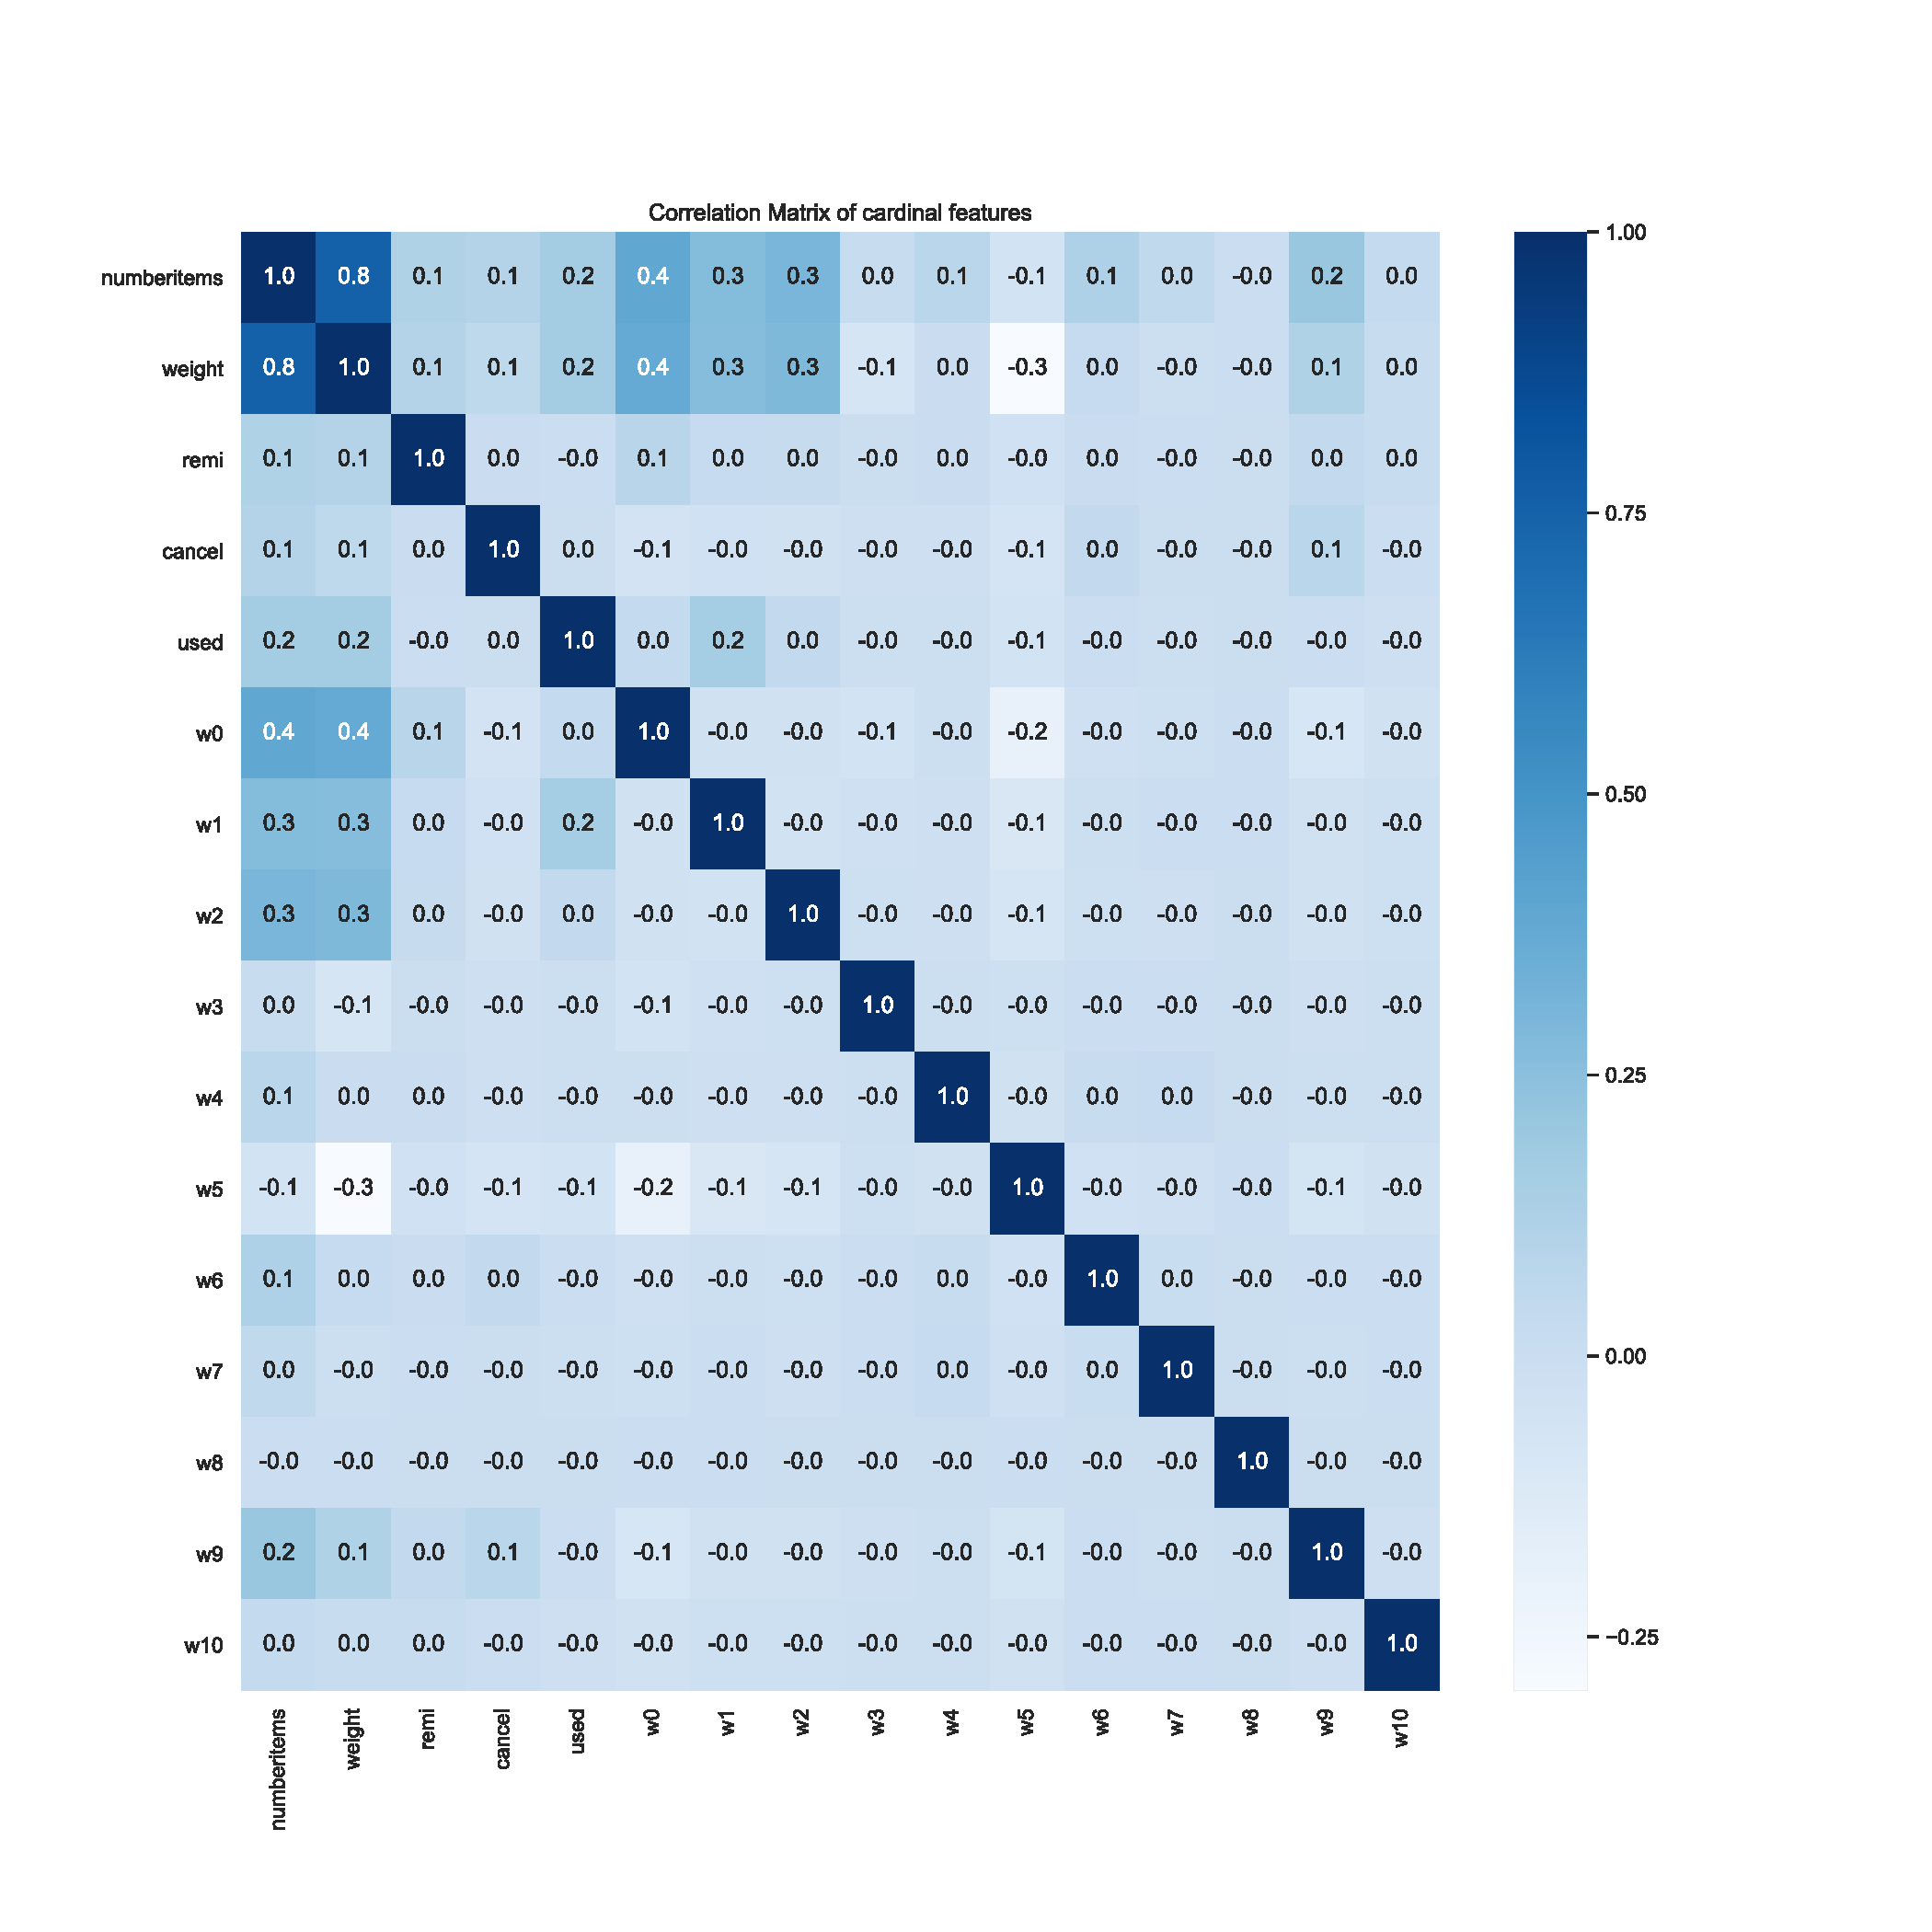
\includegraphics[scale=0.5]{pdf/correlation.pdf}
\end{center}
\caption{Korrelationsmatrix der numerischen Merkmale}
\label{fig:corr}
\end{figure}
\FloatBarrier

\subsubsection{PCA}
\label{sec:PCA}

Eine Technik, um hochdimensionale numerische Merkmale zu visualisieren ist die Hauptkomponentenanalyse (PCA). Mit dieser Methode kann ein hochdimensionaler Merkmalsraum in einen Raum niedrigerer Dimension projiziert werden. Es findet dabei eine Verschiebung der Achsen in die Richtung der maximalen Streuung statt. Zur Visualisierung können dann jeweils 2 Hauptkomponenten genutzt werden. In Abbildung \ref{fig:pca} sind zur Visualisierung die ersten beiden Hauptkomponenten genutzt worden. Diese erklären unter allen anderen Hauptkomponenten den größten Anteil der Varianz. Als wichtige Vorbereitung müssen die Merkmale zunächst standardisiert werden. Das heißt die Daten werden so skaliert, dass sie einen Mittelwert von 0 und eine Varianz von 1 besitzen. \\

In unserem Datensatz sind 16 numerische Merkmale verblieben, welche auf einen zweidimensionalen Unterraum projiziert worden sind. Dabei ist zu bemerken, dass die zwei visualisierten Hauptkomponenten nicht zwingend eine spezielle Bedeutung haben. Diese zwei Hauptkomponenten repräsentieren hauptsächlich die beiden Dimensionen mit der stärksten Varianz. Der Anteil der erklärten Varianz besagt, wie viel Information in Form von Streuung (Varianz) durch die einzelnen Hauptkomponenten erklärt werden kann. In unseren Daten erklären 2 Hauptkomponenten lediglich rund 22 \% der Streuung. \\

Bei der Visualisierung des zweidimensionalen Unterraums stellt sich heraus, dass sich die Klassengebiete stark überlappen. Nicht disjunkte Klassengebiete erhöhen die Schwierigkeit der eindeutigen Identifikation der Klassen.  Diese Beobachtung deutet darauf hin, dass ausschließlich die numerischen Merkmale keine sehr große Klassifikationsgüte versprechen und die Hinzunahme der kategorischen Merkmale wichtig ist. Es kann deshalb davon ausgegangen werden, dass Klassifikatoren, welche alle Merkmalstypen berücksichtigen, bessere Resultate liefern. Diese Vermutung wird im weiteren Verlauf mit der Anwendung des k-Nearest-Neighbor Verfahrens überprüft. Dieser Algorithmus wird alleine auf Basis der numerischen Merkmale trainiert. Anschließend wird das Verfahren mit baumartigen Algorithmen verglichen. Diese können sowohl mit numerischen, als auch mit kategorischen Merkmalen gleichzeitig umgehen.\\

In Abbildung \ref{fig:pca2} ist zusätzlich dargestellt, welchen Anteil der Varianz die einzelnen Hauptkomponenten erklären. Dabei wird besonders deutlich, dass bis auf die erste Hauptkomponente alle weiteren Hauptkomponenten einen ähnlichen Varianzanteil erklären. Dieser individuelle Anteil fällt sehr gering aus. Es sind fast alle Hauptkomponenten nötig, um über 95\% der Varianz zu erklären. Es wird deshalb im weiteren Verlauf darauf verzichtet, die numerischen Merkmale für die Klassifikation in einen niedriger dimensionalen Unterraum zu projizieren.\\

\begin{figure}[!htbp]
\begin{center}
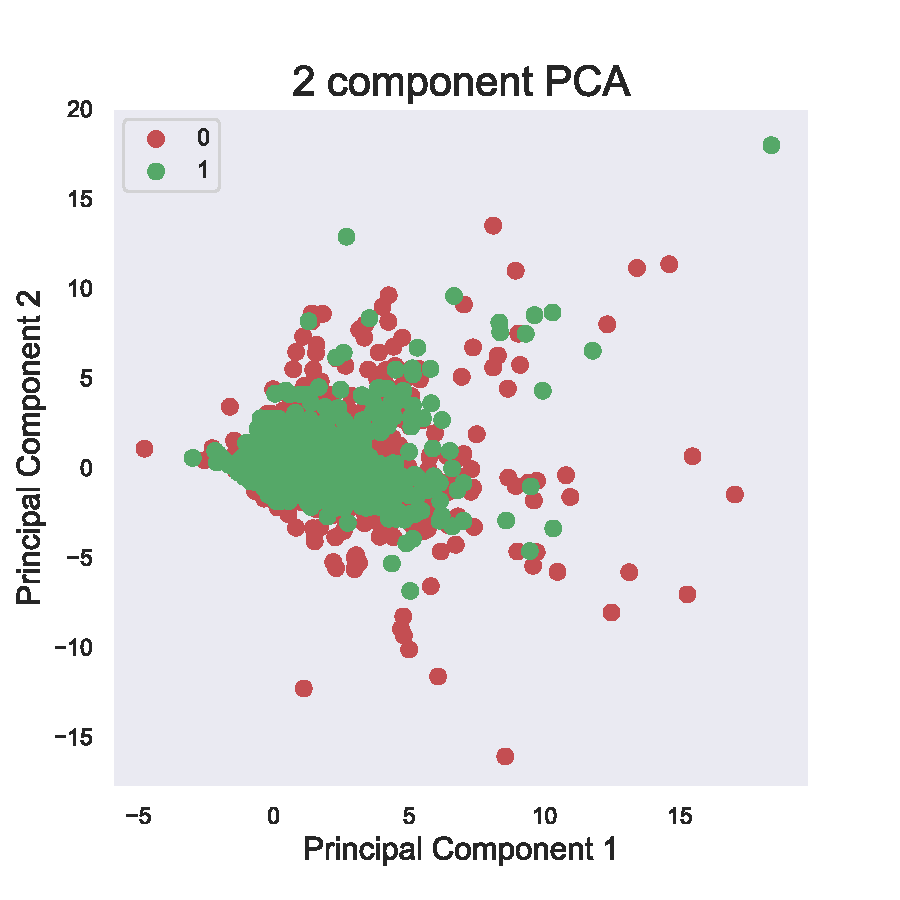
\includegraphics[scale=0.5]{pdf/pca.pdf}
\end{center}
\caption{Zwei Hauptkomponenten mit Klassenlabel}
\label{fig:pca}
\end{figure}

\begin{figure}[!htbp]
\begin{center}
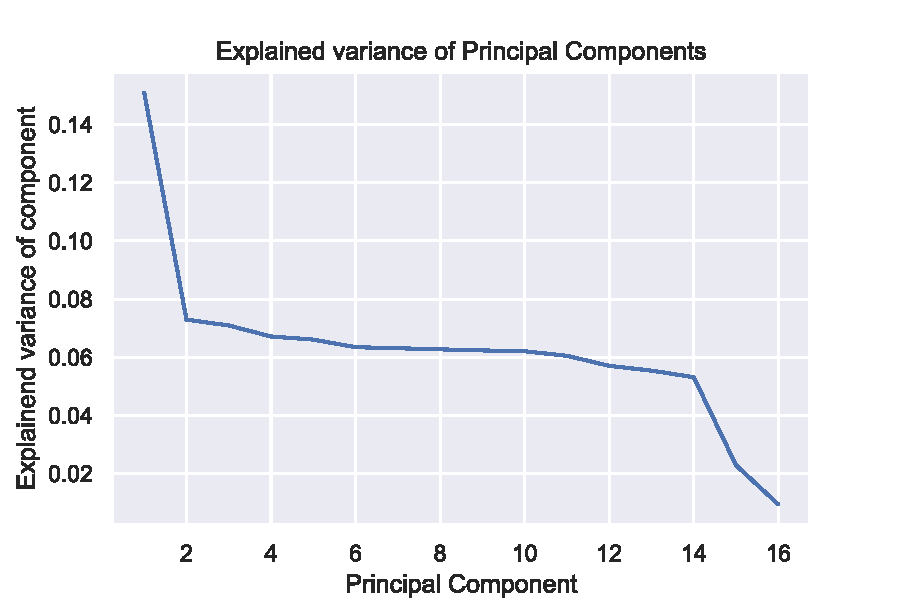
\includegraphics[scale=0.5]{pdf/pca2.pdf}
\end{center}
\caption{Hauptkomponente und erklärte Varianz}
\label{fig:pca2}
\end{figure}


\FloatBarrier
\section{Data Preparation}
\label{sec:preparation}
In der Data Preparation Phase geht es darum, die vorliegenden Daten so zu transformieren, dass am Ende dieser Phase ein Modell auf den Trainingsdaten trainiert werden kann und eine möglichst präzise Klassenvorhersage für die Testdaten erreicht wird. Unser Ziel ist die Entwicklung einer geeigneten Preprocessing Pipeline. Das bedeutet konkret, dass Transformationsschritte gewählt werden, welche in einer Funktion festgehalten werden. Diese Vorverarbeitungsfunktion sorgt dafür, dass die eingelesenen Trainings- und Testdaten so modifiziert werden, dass sie sich in einer optimalen Form für den entsprechenden Klassifikationsalgorithmus befinden. Die Entwicklung und Optimierung dieser Pipeline ist im Sinne des CRISP-DM Modells kein linearer Prozess. Stattdessen können die Vorverarbeitungsschritte anhand der Evaluation der Klassifikationsergebnisse angepasst werden.

\subsection{Feature Engingeering}
Einer der Schritte der Data Preparation Phase ist einerseits das Löschen irrelevanter Features. Andererseits wird beim Feature Engineering versucht neue, aussagekräftigere Merkmale aus den bestehenden zu erzeugen oder bestehende so zu bearbeiten, dass sie bestmöglich für den nachgeschalteten Klassifikationsalgorithmus geeignet sind. Im Folgenden werden die neu konstruierten Merkmale beschrieben:
\subsubsection{Konstruierte Attribute}
\textbf{deliverydiff:}\\

Unter den kardinalskalierten Merkmalen befindet sich unter anderem das versprochene Lieferdatum (deliverydatepromised) und das tatsächliche Lieferdatum (deliverydatereal). Ein Datum kann nicht ohne weiteres direkt für einen Klassifikationsalgorithmus wie z.B. den k-Nearest-Neighbor-Algorithmus verwendet werden. Denn bei den meisten Verfahren, werden Punkte anhand eines Ähnlichkeitsmaßes klassifiziert. Diese Algorithmen können nicht mit Datumswerten rechnen.\\ 

Deshalb bietet es sich an dieser Stelle an, aus der Differenz zwischen dem versprochenen Lieferdatum und dem tatsächlichen Lieferdatum die Lieferverzögerung zu berechnen. Dafür sind die beiden Merkmale zunächst von einem String- in ein Datums-Datentyp umgewandelt worden. Anschließend wird über eine Datumsfunktion die Differenz in Tagen ermittelt. Auffällig an den Merkmalsausprägungen des realen Lieferdatums ist das Vorkommen des Datums 0000-00-00. Dieses Datum kommt in den Trainingsdaten 1741 mal vor. Weitere Untersuchungen haben gezeigt, dass dieses Datum eingetragen wird, wenn digitale Produkte gekauft worden sind. Diese Werte werden auf den 01.01.2100 gesetzt. Dadurch entsteht eine sehr große Differenz, welche anschließend auf 0 gesetzt wird. Durch die Regel, dass Differenzen größer oder kleiner 1000 auf 0 gesetzt werden, gelingt zudem die Behandlung von falschen Einträgen wie beispielsweise das Datum 01.10.4746. Das neu generierte Merkmal ist kardinalskaliert und wird als Ganzzahl gespeichert. Es soll dabei helfen die Kundenzufriedenheit zu repräsentieren.\\

\textbf{accountdur:}\\

Ebenfalls aus einer Datumsdifferenz in Tagen, ist das Merkmal accountdur erstellt worden. Dieses Merkmal gibt die Anzahl in Tagen vom Datum der Erstbellung des Accounts bis zur ersten Bestellung im Shop an. Das neue Merkmal ist ebenfalls kardinalskaliert und nimmt ganzzahlige positive Werte an.\\

\textbf{books:}\\

Aus den Features w0 bis w5 ist das Merkmal books erstellt worden. Das Merkmal gibt die Anzahl der gekauften Artikel an, welche indirekt zur Artikelgruppe der Bücher gehören. Es werden also die bestellten gebundenen Bücher, Taschenbücher, Schulbücher, eBooks und Hörbücher aggregiert. Diese Aggregation ist deshalb gewählt worden, weil aus den Daten und der Beschreibung des Online-Händlers hervorgegangen ist, dass Buchartikel die Hauptartikelgruppe sind. Zudem hat sich aus dem Data Understanding ergeben, dass der Median der Artikel w1 bis w5 null beträgt. Durch die Aggregation wird sich eine größere Aussagekraft versprochen. \\

\textbf{nobooks:}\\

Als Pendant zu den Buchartikeln ist das Merkmale nobooks erstellt worden. Das neu konstruierte Feature aggregiert alle Artikel, welche keine unmittelbaren Buchartikel sind. Es gibt die summierte Anzahl der bestellten Filme, Musik- und Hardwareartikel sowie andere Artikel und Hardware betreffende Artikel an (w6 bis w10). \\

\textbf{Itemseff:}\\

Aus der Anzahl der bestellten Artikel, abzüglich der stornierten und zurückgegebenen Artikel, wird die Anzahl der tatsächlich gekauften Artikel erstellt (itemseff). Dieses Merkmal gibt an, wie viele Artikel effektiv durch den Kunden gekauft worden sind.

\subsubsection{Modifizierte Attribute}

\textbf{OneHotEncoding:}\\

Algorithmen des maschinellen Lernens können nicht unmittelbar mit kategorialen Merkmalen arbeiten. Damit trotzdem Modelle mit diesen Features trainiert werden können, müssen die Ausprägungen der Merkmale zunächst in einen ganzzahligen Wert codiert werden. Damit die Merkmale anschließend nicht als numerisches Merkmal interpretiert werden ist One Hot Encoding nötig.\\

Beim One Hot Encoding wird aus den codierten Merkmalen ein Binärer Vektor erstellt. Die Ausprägungen werden dadurch repräsentiert, dass nur die Spalte des Merkmals den Wert 1 annimmt und die anderen Spalten 0 werden. Besonders deutlich wird dies im Teil Modeling. Die dort trainierten Entscheidungsbäume (CART) nutzen nur binäre Splits. Die binären Splits treffen Entscheidungen anhand von „größer gleich oder kleiner gleich“ Beziehungen. Beispielsweise ist die Variable domain bereits codiert in Zahlen von 0 bis 12. Die einzelnen Ausprägungen repräsentieren die Domain des Email Providers. Das Merkmal ist nominalskaliert, sodass keine Rangfolge der Ausprägungen gebildet werden darf. Ohne One Hot Encoding könnte ein Entscheidungsbaum die Frage erstellen, ob die Domain größer gleich 6 ist. Dabei enthält man keine Fehlermeldung, jedoch entstehen falsche Ergebnisse und Fehlinterpretationen. Auf die nachfolgenden kategorialen Variablen wird deshalb One Hote Encoding angewendet, um richtige Ergebnisse zu gewährleisten.\\

\textbf{advertisingdatacode:}\\

Das Merkmal gibt an, welcher Werbecode bei der Bestellung benutzt worden ist. In den Trainingsdaten ist über 8000 mal kein Code verwendet worden. Die anderen Ausprägungen sind über 20 verschiedene Codes. Dieses nominalskalierte Merkmal ist in dieser Form für einen Klassifikator ungeeignet. Ziel ist es, die Werte zu codieren, um sie benutzbar zu machen. Möglich wäre es jede Ausprägung als Ganzzahl zu codieren und anschließend One Hot Encoding anzuwenden. Das Problem an dieser Vorgehensweise ist, dass infolgedessen über 20 neue Spalten in den Trainingsdaten erzeugt werden würden. Darüber hinaus gibt es in den Trainingsdaten weniger Ausprägungen der Variable. Dadurch entsteht eine Inkonsistenz bezüglich der Spaltenanzahl zwischen Trainings- und Testdaten. Diese Inkonsistenzen erzeugen Fehlermeldungen bei der Klassifikation. Aufgrund der obigen Erläuterung werden die Ausprägungen nur mit 0 und 1 codiert und geben an, ob ein Code vorhanden ist oder nicht. Es muss keine weitere Spalte erzeugt werden und das Feature ist für das Trainieren eines Klassifikators geeignet.\\

\textbf{salutation:}\\

Die Anrede des Kunden nimmt drei Ausprägungen an. Ein Kunde wird als männlich, weiblich oder als Firmenkunde erfasst. Das Merkmal ist bereits im Datensatz als Ganzzahl repräsentiert. Aufgrund des nominalen Skalenniveaus und der Überschreitung von zwei Ausprägungen wird das Merkmal durch One Hot Encoding transformiert. Es entstehen daher die drei neuen Spalten salutation0, salutation1 und salutation2.\\

\textbf{model:}\\

Die Bedeutung des Features model ist nicht genauer spezifiziert. Wir können dennoch nicht daraus schließen, dass das Merkmal unbedeutsam für die Klassifikationsgüte ist. Das Merkmal nimmt ebenfalls drei Ausprägungen an. Die Ausprägungen sind bereits als Ganzzahl codiert und deshalb ist nur noch die Vektorisierung des Merkmals durch One Hot Encoding nötig. Die Transformation erzeugt drei neue Spalten in unserer Merkmalsmatrix. Inwiefern das Merkmal tatsächlich Relevanz hat, wird bei einer Feature Selection im Evaluationsteil bewertet. Bei großer Bedeutung kann beim Onlinehändler nachträglich noch die genaue Bedeutung erfragt werden, um besonders bei den Baum basierten Algorithmen die Interpretationsgüte der Ergebnisse zu verbessern. \\

\textbf{paymenttype:}\\

Der Zahlungstyp besitzt die vier, bereits codierten Ausprägungen Zahlung auf Rechnung, Barzahlung, Zahlung mit dem bestehenden Account und per Kreditkarte. Das Merkmal wird ebenfalls in die Merkmalsmatrix aufgenommen und zuvor mit One Hot Encoding zu vier neuen Spalten transformiert. Die neuen Spalten bekommen die Bezeichnung paymenttype0, paymenttype1, paymenttype2 und paymenttype3.\\


\subsubsection{Gelöschte Attribute}

Die Löschung eines Attributs kann sich beispielsweise daraus ergeben, dass zu viele fehlende Werte vorhanden sind oder das Attribut aus der Sicht des Business Understandings oder der Klassifikationsgüte irrelevant ist. Des Weiteren können Attribute gelöscht werden, wenn sie wegen ihres Skalenniveaus und den Ausprägungen ungeeignet für einen spezifischen Algorithmus sind. In unserem Fall basiert das Löschen am häufigsten auf der Merkmalszusammenlegung oder der mangelnden Transformierbarkeit und Aussagekraft. Gelöscht worden sind die folgenden Attribute:\\

\textbf{deliverydatereal und deliverydatepromised:}\\

Das tatsächliche Lieferdatum und das versprochene Lieferdatum werden gelöscht, weil mithilfe der beiden Daten das neue Merkmal deliverydiff erstellt worden ist. Das neue Merkmal bildet die Datumsdifferenz in Tagen ab und spiegelt den Lieferverzug wider.\\

\textbf{datecreated und date:}\\

Aus dem Datum der Accounteröffnung datecreated und dem Datum der Erstbestellung date wird das Merkmal accountdur konstruiert. Dieses gibt die Anzahl der Tage von der Accounteröffnung bis zur ersten Lieferung an. Das neue Merkmal hat zur Folge, dass die beiden genannte Merkmale gelöscht werden.\\

\textbf{customernumber:}\\

Die Kundennummer wird gelöscht, weil sie aufgrund ihrer Individualität keine Gruppierung bezüglich der beiden Klassen ermöglicht.\\

\textbf{invoicepostcode und delivpostcode:}

Diese beiden Merkmale geben die Rechnungs- und Lieferadresse an. Beide Merkmale werden gelöscht. Der Grund liegt darin, dass die Transformation in eine Ganzzahl und anschließendes One Hot Encoding zu zahlreichen neuen Spalten der Merkmalsmatrix führen würden. Mit den unterschiedlichen Ausprägungen in Trainings- und Testdaten geht zudem eine Inkosistenz in der Spaltenanzahl beider Matrizen einher. \\

\textbf{domain:}\\

Wie bereits bei der Einführung von One Hot Encoding erwähnt, würden aus der ganzzahlig codierten Domain über zehn neue Spalten entstehen. Dadurch, dass diese negative Eigenschaft des Merkmals deutlich eine vermutete Vorhersagekraft überschreitet, wird das Merkmal gelöscht.\\

\textbf{points:}\\

Das nominalskalierte Merkmal points gibt an, ob bei der Bestellung Punkte eingelöst worden sind. In der Phase des Data Understandings hat sich gezeigt, dass dieses Merkmal ausschließlich den Wert 0 annimmt. Es wird deshalb aus der Merkmalsmatrix entfernt.\\

\textbf{title:} \\

Dieses Attribut codiert die Information über einen vorhandenen Titel der Person. Konkret heißt das, dass beispielsweise ein angegebener Doktortitel mit 1 bezeichnet wird. Andernfalls nimmt das Merkmal den Wert 0 an. In Abbildung \ref{fig:distC2} sind die absoluten Häufigkeiten des Merkmals visuell dargestellt worden. Es ist zu erkennen, dass kaum eine Person einen Titel angegeben hat. Somit können die Merkmalsausprägungen nicht zur Klassenvorhersage beitragen. Daher wird dieses Merkmal entfernt.\\

\textbf{gift:}\\

Ebenso wie das Merkmal title ist die Geschenkoption nahezu nie gewählt worden. Damit wird es aus den gleichen Gründen gelöscht.\\

\pagebreak

\subsection{Resampling}
Der vorliegende Trainingsdatensatz ist, bezüglich der Zielvariable, stark unbalanciert. Das heißt, dass die relativen Klassenhäufigkeiten stark voneinander abweichen. Bei einer binären Klassifikation resultiert daraus eine Klasse, welche besonders häufig vorkommt und eine stark unterrepräsentierte Klasse. In unserem Fall hat das überrepräsentierte Label 0 (Kein Wiederkäufer) eine relative Häufigkeit von ca. 81 \% und das Label 1 (Wiederkäufer) tritt in ca. 19 \% der Fälle auf.\\

 Infolge eines nicht balancierten Trainingsdatensatzes entsteht die Problematik, dass die Güte des Klassifikators fehlinterpretiert werden kann. Ein Klassifikator prognostiziert bei unbalancierten Klassen vermehrt das überrepräsentierte Klassenlabel. Ist dann die Verteilung der Klassen in den Testdaten ähnlich zur Trainingsdatenverteilung führt das zu einer hohen Genauigkeit (Accuracy Score). Beispielsweise sind in unseren Testdaten rund 80 \% der Kunden mit der Ausprägung 0 etikettiert. Ein Klassifikator, welcher ausschließlich das Label 0 vorhersagt, liegt infolgedessen in 80 \% der Fälle richtig. Daraus resultiert unmittelbar ein Accuracy Score von 80 \%. Ohne die Hinzunahme weiterer Kennzahlen wird die Leistung des Klassifikators überschätzt.\\
 
Werden anschließend Kennzahlen wie Precision und Recall berechnet, wird ersichtlich, dass das unterrepräsentierte Klassenlabel nicht oft wiedergefunden wird (niedriger Recall). Es kann sich für die unterrepräsentierte Klasse sogar ein Recall von 0 \% ergeben, weil diese Klasse nie vorhergesagt wird. Um diese Problematik zu lösen ist die Anpassung der Gewichtung der Klassen nötig.\\

Eine einfache Möglichkeit, um eine gleiche Klassenverteilung herzustellen ist das Resampling. Beim Resampling wird in der einfachsten Form zwischen Over – und Undersampling unterschieden. Beim Oversampling werden Dateneinträge der Minderheitsklasse zufällig mit Zurücklegen gezogen und in die Trainingsdatenbasis eingefügt. Die Größe des Trainingsdatensatzes wird artifiziell erhöht. Undersampling stellt die Gleichverteilung durch Löschen von Einträgen der Mehrheitsklasse her. Beide Strategien haben Vor- und Nachteile. Oversampling kann Overfitting verursachen, weil Einträge der Trainingsdaten einfach kopiert werden. Undersampling führt dagegen zu einem Informationsverlust, durch das Löschen von Einträgen. Aufgrund der begrenzten Trainingsdatengröße ist die Entscheidung deshalb auf Oversampling gefallen.\\ 

In Abbildung \ref{fig:over} wird die Verteilung der Merkmale in Trainings- und Testdaten nach dem Oversampling dargestellt. Die Trainingsdaten weisen jetzt eine Gleichverteilung bezüglich der beiden Klassen auf. Die Testdaten bleiben von Resampling Methoden unberührt. Klassifikatoren wie der kNN-Algorithmus lernen die Trainingsdaten auswendig. Folglich würden sie die artifiziell erzeugten Einträge richtig klassifizieren und die Klassifikationsgüte positiv verfälschen.

\begin{figure}[!htbp]
\begin{center}
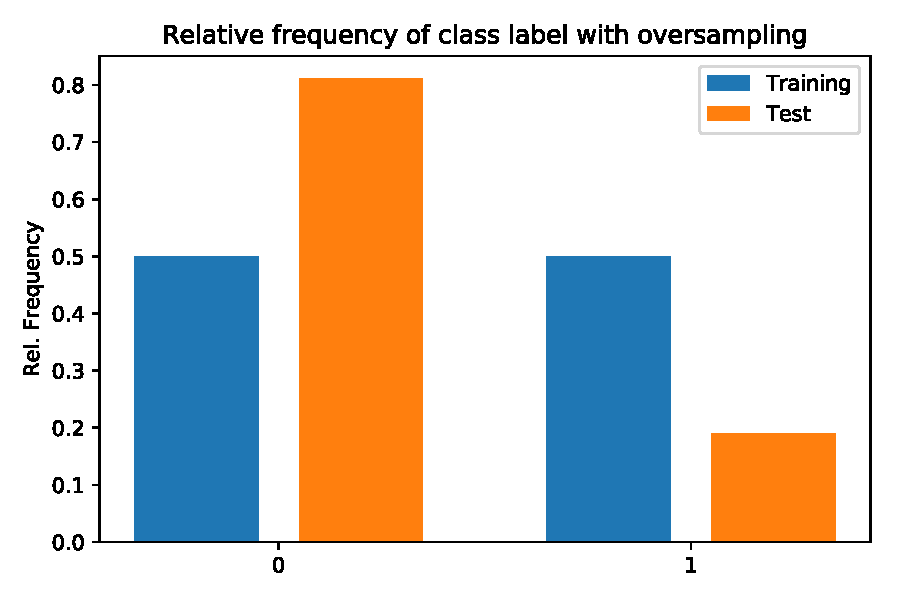
\includegraphics[scale=0.5]{pdf/classDistOver.pdf}
\end{center}
\caption{Klassenverteilung nach Oversampling der Minderheitsklasse}
\label{fig:over}
\end{figure}

\FloatBarrier

\subsection{Merkmalsskalierung}
\label{sec:Skalierung}

Der finale und gleichzeitig einer der wichtigsten Schritte der Data Preparation Phase ist das Skalieren von Merkmalen. Das bedeutet, dass der unterschiedlich ausfallende Wertebereich der kardinalskalierten Merkmale auf einen einheitlichen Wertebereich abgebildet wird. Eine unterschiedliche Skalierung kann dafür sorgen, dass bei distanzbasierten Verfahren wie dem kNN-Algorithmus Merkmale mit größeren Ausprägungen des Wertebereichs stärker gewichtet werden.\\

Die beiden bekanntesten Verfahren zur Skalierung der Merkmale ist die Standardisierung und die Min-Max-Skalierung. Bei der Standardisierung werden die Merkmale auf einen Mittelwert von 0 und eine Varianz von 1 normiert. Das wird dadurch erreicht, dass von jeder Ausprägung der Mittelwert abgezogen und anschließend durch die Varianz des Merkmals geteilt wird. Bei der Min-Max-Skalierung wird der Wertebereich so verschoben, dass die kleinste Ausprägung den Wert 0 und die größte den Wert 1 besitzt. Alle anderen Ausprägungen liegen dazwischen. Diese Transformation wird erzeugt, indem die Differenz der Ausprägung zum Minimum berechnet und anschließend durch die Spannweite von Minimum und Maximum geteilt wird. In der Phase des Data Understandings ist ersichtlich geworden, dass die numerischen Merkmale linkssteil und rechtsschief sind. Es liegt keine symmetrische Verteilung vor. Visuell wird deshalb die Normalverteilungsannahme abgelehnt. Aus diesem Grund wird als Skalierungsverfahren die Min-Max-Skalierung für das weitere Vorgehen gewählt.
\pagebreak

\section{Modeling}

Algorithmen des Data Minings und Maschinellen Lernens lassen sich in die übergeordneten Kategorien des überwachten und unüberwachten Lernens unterteilen. Beim Überwachten Lernen sind die Klassenlabel, also die Ausprägungen der Zielvariable, bekannt. Innerhalb des überwachten Lernens wird zwischen Klassifikation und Regression unterschieden. Ziel der Regression ist das Schätzen der numerischen Zielvariable auf Basis der vorhandenen Merkmale.\\

Bei der reinen Klassifikation sind die Klassenlabel in der Regel kategorische Merkmale. Beziehungsweise werden sie durch eine geeignete Transformation kategorisiert. In der gegebenen Aufgabenstellung geht es darum vorherzusagen, ob ein Kunde innerhalb von 90 Tagen erneut im Onlineshop einen Einkauf tätigt. Damit ist ein Kunde entweder ein Wiederkäufer (1) oder nicht (0). Für die Testdaten soll dieses Etikett prognostiziert werden. Damit handelt es sich um überwachtes Lernen. Dadurch, dass die vorhandenen Klassenlabel nur zwei Kategorien aufweisen, wird diese Aufgabenstellug auch als binäre Klassifikation bezeichnet.\\

Ziel ist es einen entsprechenden Algorithmus zu entwickeln, welcher, unter Berücksichtigung möglichst aussagekräftiger Merkmale, Regeln zur Einteilung der Klassengebiete erlernt. Das Trainieren des Modells wird mithilfe der Trainingsdaten bewerkstelligt. Auf die Testdaten werden die gelernten Regeln angewendet, um das für den Klassifikator unbekannte Klassenlabel zu ermitteln. Die Evaluation findet mit den tatsächlichen Labeln der Testdaten und der gegeben Kostenmatrix statt. Trainings- und Testdaten sind bereits zuvor aufgeteilt worden. Es sind deshalb keine weiteren Splits nötig.\\

Neben qualitativ hochwertigen Daten, ist die Auswahl eines geeigneten Algorithmus wichtig. Im Folgenden werden die vier Klassifikationsalgorithmen kurz beschrieben, welche beim Trainieren und Testen genutzt worden sind. Dabei ist die Reihenfolge in aufsteigender Komplexität des Verfahrens gewählt worden. 

\subsection{k-Nearest-Neighbor-Algorithmus}
\label{sec:kNN}
Der k-Nächste-Nachbarn-Klassifikator ist ein instanzbasiertes Lernverfahren, welches die Trainingsdatenbasis auswendig lernt. Datenpunkte des Testdatensatzes werden per Mehrheitsentscheid, anhand ihrer Ähnlichkeit zu den k nächsten Nachbarn der Trainingsdaten, klassifiziert. Der Algorithmus trifft die Annahme, dass Objekte einer Klasse bezüglich ihrer Merkmalsausprägungen nah beieinander liegen.\\

 Eine Herausforderung ist die Wahl des Distanzmaßes, welches je nach Skalenniveau angepasst werden muss. Ein valides Distanzmaß, welches ohne Informationsverlust die Ähnlichkeit zwischen nominal, ordinal – und kardinalskalierte Merkmalen berechnen kann, existiert nicht. Damit unterliegt der Algorithmus Einschränkungen gegenüber baumartigen Algorithmen, wenn ein Datensatz bezüglich des Skalenniveaus sehr heterogen ist. Nichtsdestotrotz ist der Algorithmus sehr einfach anzuwenden und intuitiv verständlich, weshalb dessen Ergebnisse als erste Richtlinie dienen können. Im weiteren Verlauf ist sich für die euklidische Distanz entschieden worden.\\

Das hat zur Folge, dass ausschließlich kardinalskalierte Merkmale in die Trainingsdatenbasis aufgenommen werden. Diese müssen aufgrund des unterschiedlichen Skalenniveaus zunächst auf einen gemeinsamen Wertebereich gebracht werden. Wie im Abschnitt Merkmalsskalierung erläutert worden ist, wird dafür die Min-Max-Skalierung genutzt. Damit bewegen sich alle Ausprägungen zwischen 0 und 1. Neben dem Distanzmaß, ist die Anzahl der Nachbarn k, als weiterer Hyperparameter festzulegen. Um immer die Situation einer Mehrheit zu erreichen, wird k generell auf ungerade Werte festgelegt. Der final genutzte Wert wird durch Enumeration verschiedener Werte für k ermittelt. Dabei wird das k gewählt, welches den größten Umsatz auf den Testdaten generiert.\\


\subsection{Entscheidungsbaum Klassifikator}
\label{sec:Tree}
Im Gegensatz zum kNN-Algorithmus können Entscheidungsbäume gleichzeitig auf Merkmalen mit unterschiedlichem Skalenniveau trainiert werden. Dabei ist keine Transformation der Merkmale nötig. Zudem können Entscheidungsbäume mit nicht normierten numerischen Merkmalen umgehen. Eine Min-Max-Skalierung wird deshalb ebenfalls nicht benötigt. Entscheidungsbäume versuchen durch Splits bezüglich der Merkmalsausprägungen die Klassen voneinander zu trennen und möglichst disjunkte Klassengebiete zu erzeugen. Maße für die Reinheit des erzeugten Splits sind die Gini-Unreinheit und die Entropie. Beide Maße erzeugen ähnliche Bäume, weshalb dieses Kriterium im weiteren Verlauf nicht als entscheidungsrelevant angesehen wird.\\

Beim Trainieren von Entscheidungsbäumen wird auf die freie Software-Bibliothek Scikit-learn für die Programmiersprache Python zurückgegriffen. Diese Bibliothek verwendet den CART-Algorithmus (Classification and Regression Trees) zum Trainieren von Entscheidungsbäumen. Im Gegensatz zu anderen Algorithmen wie dem ID3 und seinem Nachfolger C4.5 verwendet dieser Baum ausschließlich binäre Splits. Wie bereits in der Data Preparation Phase beschrieben, müssen nominalskalierte Merkmale als Zahl codiert werden. Nominalskalierte Merkmale mit mehr als zwei Ausprägungen werden durch One-Hot-Encoding vektorisiert, weil der Algorithmus die Merkmale sonst als numerisch interpretiert. Das Verfahren benutzt standardmäßig die Gini-Unreinheit. Um bestmögliche Ergebnisse zu erhalten werden verschiedene Konfigurationen bezüglich der maximalen Baumtiefe auf allen Merkmalen ausgetestet. Bei der Backward Feature Elimination wird dann die Tiefe auf den vielversprechendsten Wert festgesetzt.

\subsection{Random Forests}
\label{sec:RF}

Der Random-Forest-Klassifikator basiert auf den zuvor beschriebenen Entscheidungsbäumen. Im Gegensatz zu diesen, zählt er jedoch zu einer Gruppe von Prädiktoren, welche als Ensemble Learning Methoden bezeichnet werden. Random Forests trainieren nach der Bagging Methode auf unterschiedlich, zufällig ausgewählten Teilmengen des Trainingsdatensatzes Entscheidungsbäume. Die Klassifikation der Testdaten basiert auf Mehrheitsentscheid der trainierten Gruppe von Entscheidungsbäumen. Ein weiterer Unterschied ist die Generierung von Splits. Einfache Entscheidungsbäume erstellen Splits in Form einer gierigen Suche. Es wird das Merkmal als Split genutzt, welches die geringste Unreinheit erzeugt. Der Random-Forest-Klassifikator ermittelt das beste Merkmal in einer zufälligen Untermenge von Merkmalen. Es entsteht folglich eine größere Diversität von Bäumen. Aufgrund der Ähnlichkeit zu Entscheidungsbäumen enthält der Algorithmus identische Parameter und zusätzlich Parameter eines Bagging-Klassifikators. Bei der zu wählenden Konfiguration, werden die Standardwerte genutzt und nur die Tiefe der Bäume angepasst.

\subsection{AdaBoost}
\label{sec:Ada}

AdaBoost gehört zur Klasse der Meta-Algorithmen. Der Algorithmus kombiniert schwache Klassifikatoren zu einem starken Klassifikator. Unter schwachen Klassifikatoren versteht man zum Beispiel sehr einfache Entscheidungsbäume, welche nur eine geringe Anzahl an Splits durchführen. Beim Bagging und dem oben genannten Random-Forest-Klassifikator werden Klassifikatoren parallel trainiert. Im Gegensatz dazu werden bei Boosting Algorithmen wie AdaBoost die Basisverfahren sequentiell verschaltet. In diesem sequentiellen Ablauf werden fehlklassifizierten Werten eine höhere Gewichtung zugewiesen, um diesen beim Nachfolgenden Klassifikator mehr Aufmerksamkeit zu schenken. Ebenso erhalten Klassifikatoren mit geringeren Fehlerraten höhere Gewichte bei der Entscheidungsfindung. Als Basisverfahren sind Entscheidungsbäume gewählt worden, weil diese gut mit unterschiedlichen Skalenniveaus umgehen können. Als weiterer Hyperparameter ist die Anzahl der Entscheidungsbäume variiert worden, um bestmögliche Ergebnisse zu erzielen.  

\section{Evaluation}
\label{sec:eval}
\subsection{Das Evaluationskriterium}
Zur Evaluation eines Klassifikators gibt es zahlreiche unterschiedliche Qualitätsmaße. Die Wahl eines geeigneten Qualitätsmaßes hängt unmittelbar mit der Aufgabenstellung und den sich daraus ergebenden Zielen zusammen. Generell werden diese Kennzahlen anhand der Vorhersagen auf den Testdaten berechnet. Um zufällige Effekte für die Auswertung einer Teststichprobe einzugrenzen werden die Kennzahlen oftmals mittels Kreuzvalidierung errechnet. In dieser Aufgabenstellung sind die Testdaten explizit vorgegeben. Des Weiteren befinden sich in den Trainingsdaten zahlreiche Duplikate aufgrund des künstlichen Generierens von weiteren Datenpunkte mittels Oversampling. Daher wird auf eine Kreuzvalidierung verzichtet und jegliche Form der Evaluation anhand der extern gegebenen Testdaten durchgeführt.\\

Ein leicht zugängliches Maß ist die Anzahl der korrekt klassifizierten Werte (Accuracy). Dieses Maß kann auf unbalancierten Daten leicht zu Fehlinterpretationen führen. Klassifikatoren, welche nur die unterrepräsentierte Klasse vorhersagen erreichen unmittelbar eine Genauigkeit von 80 \%, aufgrund der Testdatenverteilung. Wird jedem Kunden der Testdaten ein Gutschein versendet ergibt sich mit der zugrundeliegenden Kostenmatrix ein Umsatz von 674.50 \euro{}. Dieser Umsatz wird im weiteren Verlauf als Basisumsatz bezeichnet. Implizit repräsentiert die Kostenmatrix die Berücksichtigung von Precision und Recall.\\

Ist der Recall für die Wiederkäufer gering, so können diese nicht wiedergefunden werden. Das Nichtfinden von Wiederkäufern geht damit einher, dass ihnen ein Gutschein zugesendet wird. Das hat wiederum einen Verlust von 5 \euro{} zur Folge, weil sie auch ohne Gutschein erneut gekauft hätten. Ist die Präzision bezüglich der Nicht-Wiederkäufer gering, erhalten diese keinen Gutschein und können den Umsatz nicht erhöhen. Durch diese implizite Repräsentation von Precision und Recall durch die Kostenmatrix, wird ausschließlich der erzielte Umsatz als Gütemaß herangenzogen. Ziel ist es diesen Umsatz zu maximieren und eine Verbesserung gegenüber der Basisumsatz zu erzielen. Diesen würde das Unternehmen nämlich ohne intelligente Vergabe erreichen.


\subsection{Wahl der Hyperparameter}

Im Abschnitt über die Klassifikatoren sind die entsprechenden Hyperparameter der Verfahren genannt worden. Hyperparameter müssen vor dem eigentlichen Trainieren des Modells festgelegt werden. Dabei gibt es verschiedene Wege möglichst geeignete Hyperparameter zu finden. Mittels einer vollständigen Enumeration kann ein diskretisiertes Gitter von Parameterkombinationen durchsucht werden. Im Gegensatz zu einer vollständigen Suche können zufällige Werte ausgetestet werden. Für bestimmte Klassifikatoren können darüber hinaus mittels Gradientenverfahren lokale Optima gefunden werden.\\

Im Folgenden wird sich auf eine heuristische Auswahl beschränkt. Das heißt, es werden einige Werte vorgegeben, welche einen realistischen Wertebereich des Hyperparameters gut abbilden. Dabei werden kleine, mittlere und sehr große Werte für den Hyperparameter ausgetestet. Grundlage sind die vorverarbeiteten Trainings- und Testdaten. Es werden alle Features genutzt, welche nach der Data Preparation Phase noch vorhanden sind. Ausnahme stellt der kNN-Algorithmus dar, bei welchem nur die kardinalskalierten Merkmale genutzt worden sind.\\

In Abbildung \ref{fig:hyper} sind die Ergebnisse der einfachen Suche dargestellt. Dabei ist zu erkennen, dass der k-Nächste-Nachbarn Algorithmus trotz Wahl verschiedener Werte von k, den Basisumsatz kaum übertreffen kann. Das hängt unmittelbar mit dem Informationsverlust durch nicht Berücksichtigung aller kategorischen Merkmale zusammen. Wie vermutet, ist dieser Algorithmus für einen sehr heterogenen Datensatz ungeeignet. Nichtsdestotrotz liefert er mit einem erzielten Umsatz von über 700 \euro{} (k=5) eine erste Richtlinie. Diese sollte von weiteren Klassifikatoren mindestens erreicht werden, da diesen zusätzlich alle kategorischen Features zur Verfügung stehen.\\

Der Entscheidungsbaum Klassifikator liefert auf allen Merkmalen, mit einer maximalen Tiefe von 5, die besten Ergebnisse. Das gleiche Resultat hat sich für den Random-Forest-Klassifikator ergeben. Der AdaBoost Klassifikator generiert mit 50 Entscheidungsbäumen den höchsten Umsatz. Auffällig ist, dass der Entscheidungsbaum eine sehr große Streuung bezüglich der Wahl der Tiefe hat. Offensichtlich erzeugen zu kleine Bäume einen hohen Bias und zu tiefe Bäume neigen zur Überanpassung. Nichtsdestotrotz sind diese Ergebnisse stark von Faktoren wie dem zugrundeliegenden Datensatz abhängig. Des Weiteren unterliegen sie zufälligen Effekten wie den zufällig gezogenen Einträgen beim Oversampling oder der Qualität der Bootstrap Stichproben (Random Forest). Für generelle Aussagen sind datensatzübergreifende Simulationsstudien nötig, welche die Grenzen dieser Projektarbeit überschreiten. Nichtsdestotrotz werden die ermittelten Parameter für die nachfolgende Backward Feature Elimination ausgewählt und festgesetzt.




\begin{figure}[H]
  \centering  
  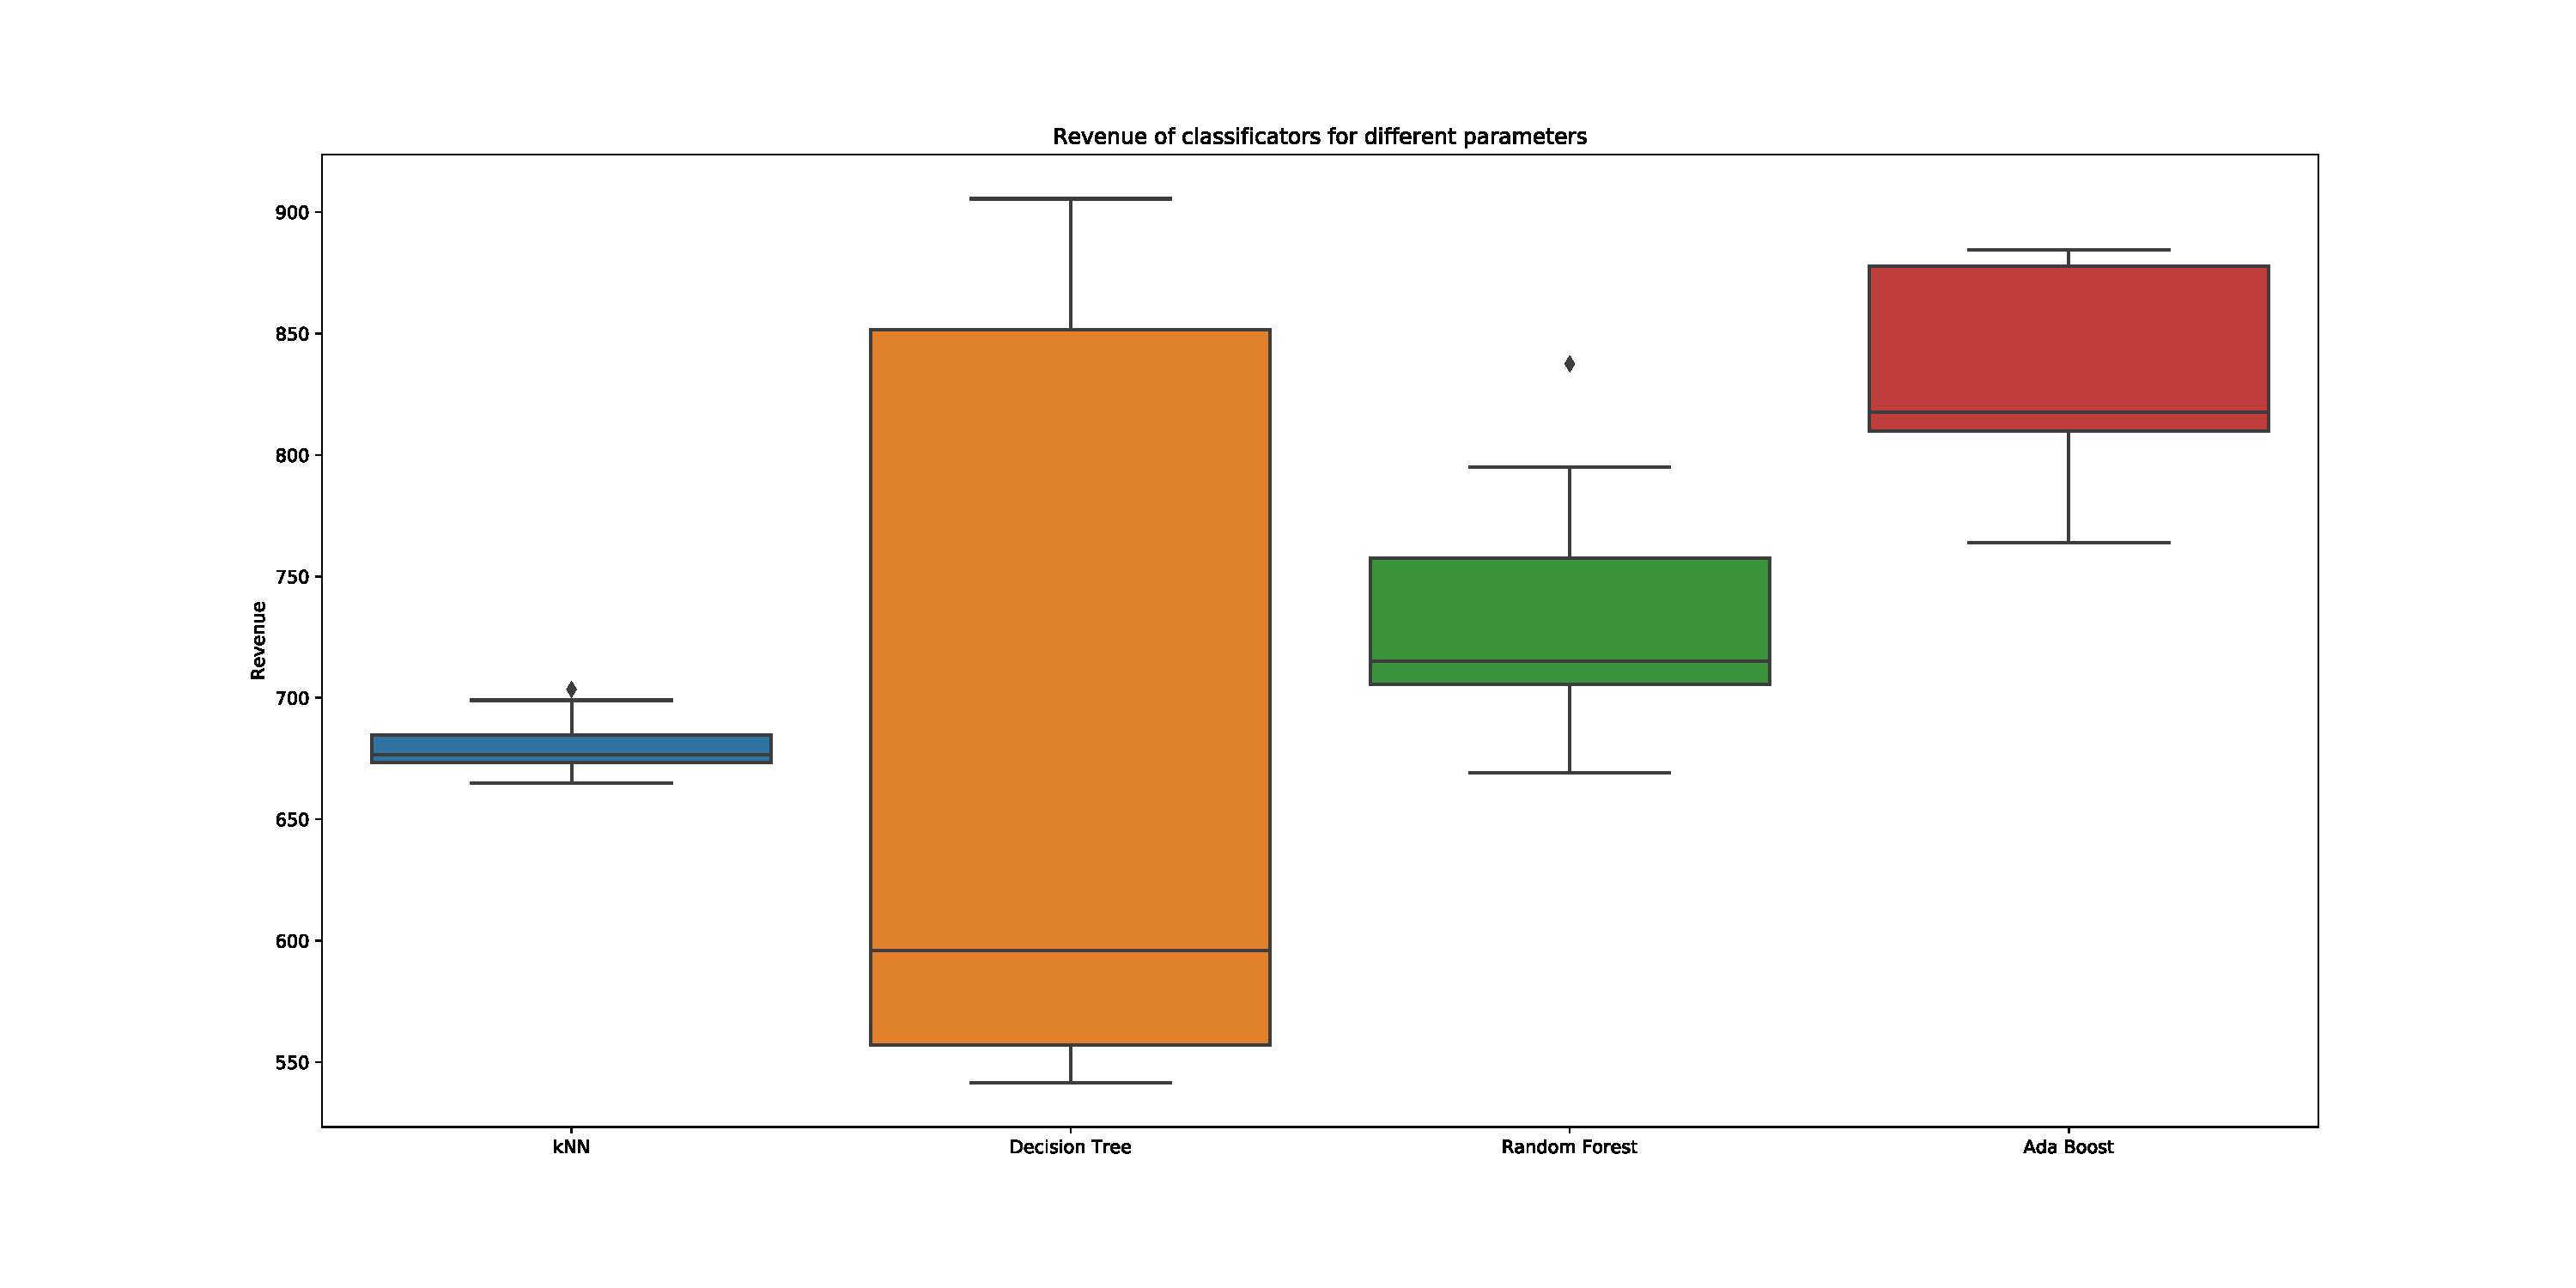
\includegraphics[scale=0.3]{pdf/hyperparameter_1.pdf}
  \caption{Variation der Hyperparameter auf dem kompletten Merkmalsraum}
  \label{fig:hyper}
\end{figure}


\subsection{Backward Feature Elimination}

Bisher ist mit der kompletten Datenmatrix und einem Entscheidungsbaum Klassifikator ein Umsatz von über 900 \euro{} erreicht worden. Im nächsten Schritt soll mittels Backward Feature Elimination die Anzahl der Merkmale variiert werden. Damit wird getestet, ob durch vielversprechende Merkmalskombinationen ein neues Umsatzmaximum ermittelt werden kann. Zum anderen wird ersichtlich, wie das Wegnehmen von Merkmalen das Klassifikationsergebnis beeinflusst. Aufgrund des Fluchs der Dimension ist ein kleinerer Merkmalsraum generell zu bevorzugen. Darüber hinaus ergibt sich eine Rangfolge der entfernten Features. Dadurch wird indirekt die Wichtigkeit eines Merkmals anhand verschiedener Klassifikatoren ermittelt. Auch aus unternehmerischer Sicht ist die Ermittlung der wichtigsten Merkmale relevant. Somit kann gezielt versucht werden diese so zu beeinflussen, dass der Onlineshop mehr Kunden zum Wiederkauf anregen kann. Losgelöst von der Gutscheinaktion, ergäbe sich dadurch ein höherer Umsatz.\\

Die Backward Feature Elimination ist für die baumartigen Algorithmen durchgeführt worden. Bei diesem Verfahren wird ein Klassifikator zunächst auf allen Features trainiert. In jeder Iteration wird ein Feature entfernt. Die Ermittlung, welches Merkmal entfernt wird, geschieht durch das sequentielle Weglassen eines Merkmals der noch vorhandenen Merkmale. Nachdem jedes Merkmal einmal weggelassen worden ist, wird der maximale Umsatz der Iteration ermittelt. Dieser Maximale Umsatz ist folglich ohne das weggelassene Merkmal entstanden. Es kann deshalb entfernt werden. Diese Prozedur wird solange wiederholt, bis nur noch ein Merkmal vorhanden ist.\\

\FloatBarrier
\begin{figure}[!htbp]
\begin{center}
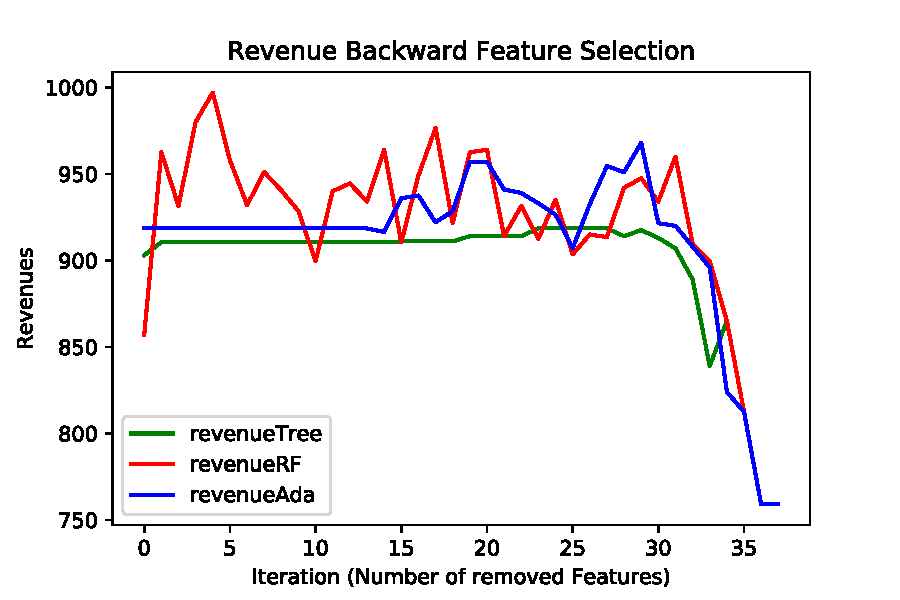
\includegraphics[scale=0.8]{pdf/backward2.pdf}
\end{center}
\caption{Umsatz in Anbhängigkeit zur Anzahl der entfernten Merkmale}
\label{fig:backward2}
\end{figure}
\FloatBarrier

In Abbildung \ref{fig:backward2} sind die sich ergebenden Umsätze in Abhängigkeit von der Anzahl der entfernten Merkmale abgebildet. Es ist zu erkennen, dass die drei Algorithmen, trotz des Entfernens von bis zu 30 Merkmalen, immer noch Umsätze von über 900 \euro{} erzielen. Den größten Wert erzielt der Random-Forest-Klassifikator mit 33 Merkmalen. Dabei wird ein Umsatz von 997 \euro{} erzeugt. (Die exakten Werte befinden sich in Tabelle \ref{table: Backward}) Zudem wird deutlich, dass die beiden Ensemble Methoden größere Umsätze erzielen als der einfache Entscheidungsbaum Klassifikator. Auffällig ist, dass der Entscheidungsbaum bis zur Entfernung von 32 Merkmalen sehr konstante Umsätze erzielt. Es kann angenommen werden, dass der konstante Umsatz mit der maximalen Tiefe von 5 zusammenhängt. Der Entscheidungsbaum erzeugt die Splits anhand einer gierigen Suche. Sind die besten Splits gewählt und werden die entsprechenden Merkmale nicht entfernt, so ändert sich der Baum nicht. Die deutlich größeren Schwankungen beim Random-Forest-Klassifikator lassen sich vermutlich auf die zufälligen Effekte bei der Bildung der Bäume mittels Bootstrap Stichproben und der zufälligen Merkmalsauswahl zurückführen. Auch hier wäre eine genauere Untersuchung mithilfe einer Simulationsstudie nötig, um diese Vermutungen zu bestätigen.\\ 

In Tabelle \ref{table: Backward} werden die Ergebnisse der Backward Feature Elimination ausführlich dargestellt. Für jeden Algorithmus ist das entfernte Feature der Iteration (Iter.) angegeben. Die Iteration entspricht der Anzahl der entfernten Merkmale. Außerdem ist der erzielte Umsatz (Rev.) ausgewiesen, der ohne dieses Merkmal erreicht wird. Alle drei Algorithmen überschneiden sich bezüglich der beiden wichtigsten Merkmale. Diese sind Newsletter und die Anzahl der zurückgesendeten Artikel (remi). Es überrascht nicht, dass diese beiden Merkmale hohe Aussagekraft besitzen. Das Abonnieren eines Newsletters ist eine erste Kundenbindungsmaßnahme und kann dafür sorgen, dass Kunden erneut beim Händler bestellen. Die Vermutung, welche im Teil Data Understanding visuell hergeleitet worden ist, bestätigt sich somit. Die Anzahl der zurückgesendeten Artikel kann als Indiz für die Unzufriedenheit mit den bestellten Artikeln angesehen werden. Schickt ein Kunde viele Artikel zurück, ist er möglicherweise nicht mit der Qualität einverstanden oder er hat falsche Artikel erhalten. \\

Sehr früh entfernen alle Klassifikatoren die Unterschiedlichen Zahlungstypen (paymenttype) und das nicht weiter spezifiziert Merkmal model. Nichtsdestotrotz gibt es auch Inkonsistenzen bezüglich der entfernten Merkmale. Der Entscheidungsbaum und Random-Forest-Klassifikator behalten bis zur 36. Iteration das Merkmal deliverytype, während diese beim AdaBoost bereits in der 19. Iteration entfernt wird. Die Backward Feature Elimination hat dazu beigetragen einen neuen besten Klassifikator zu finden, welcher einen Umsatz von fast 1000 \euro{} erreicht. Dieser Klassifikator soll im nächsten Teil ausführlich evaluiert werden.


%\begin{figure}[H]
%  \centering  
%  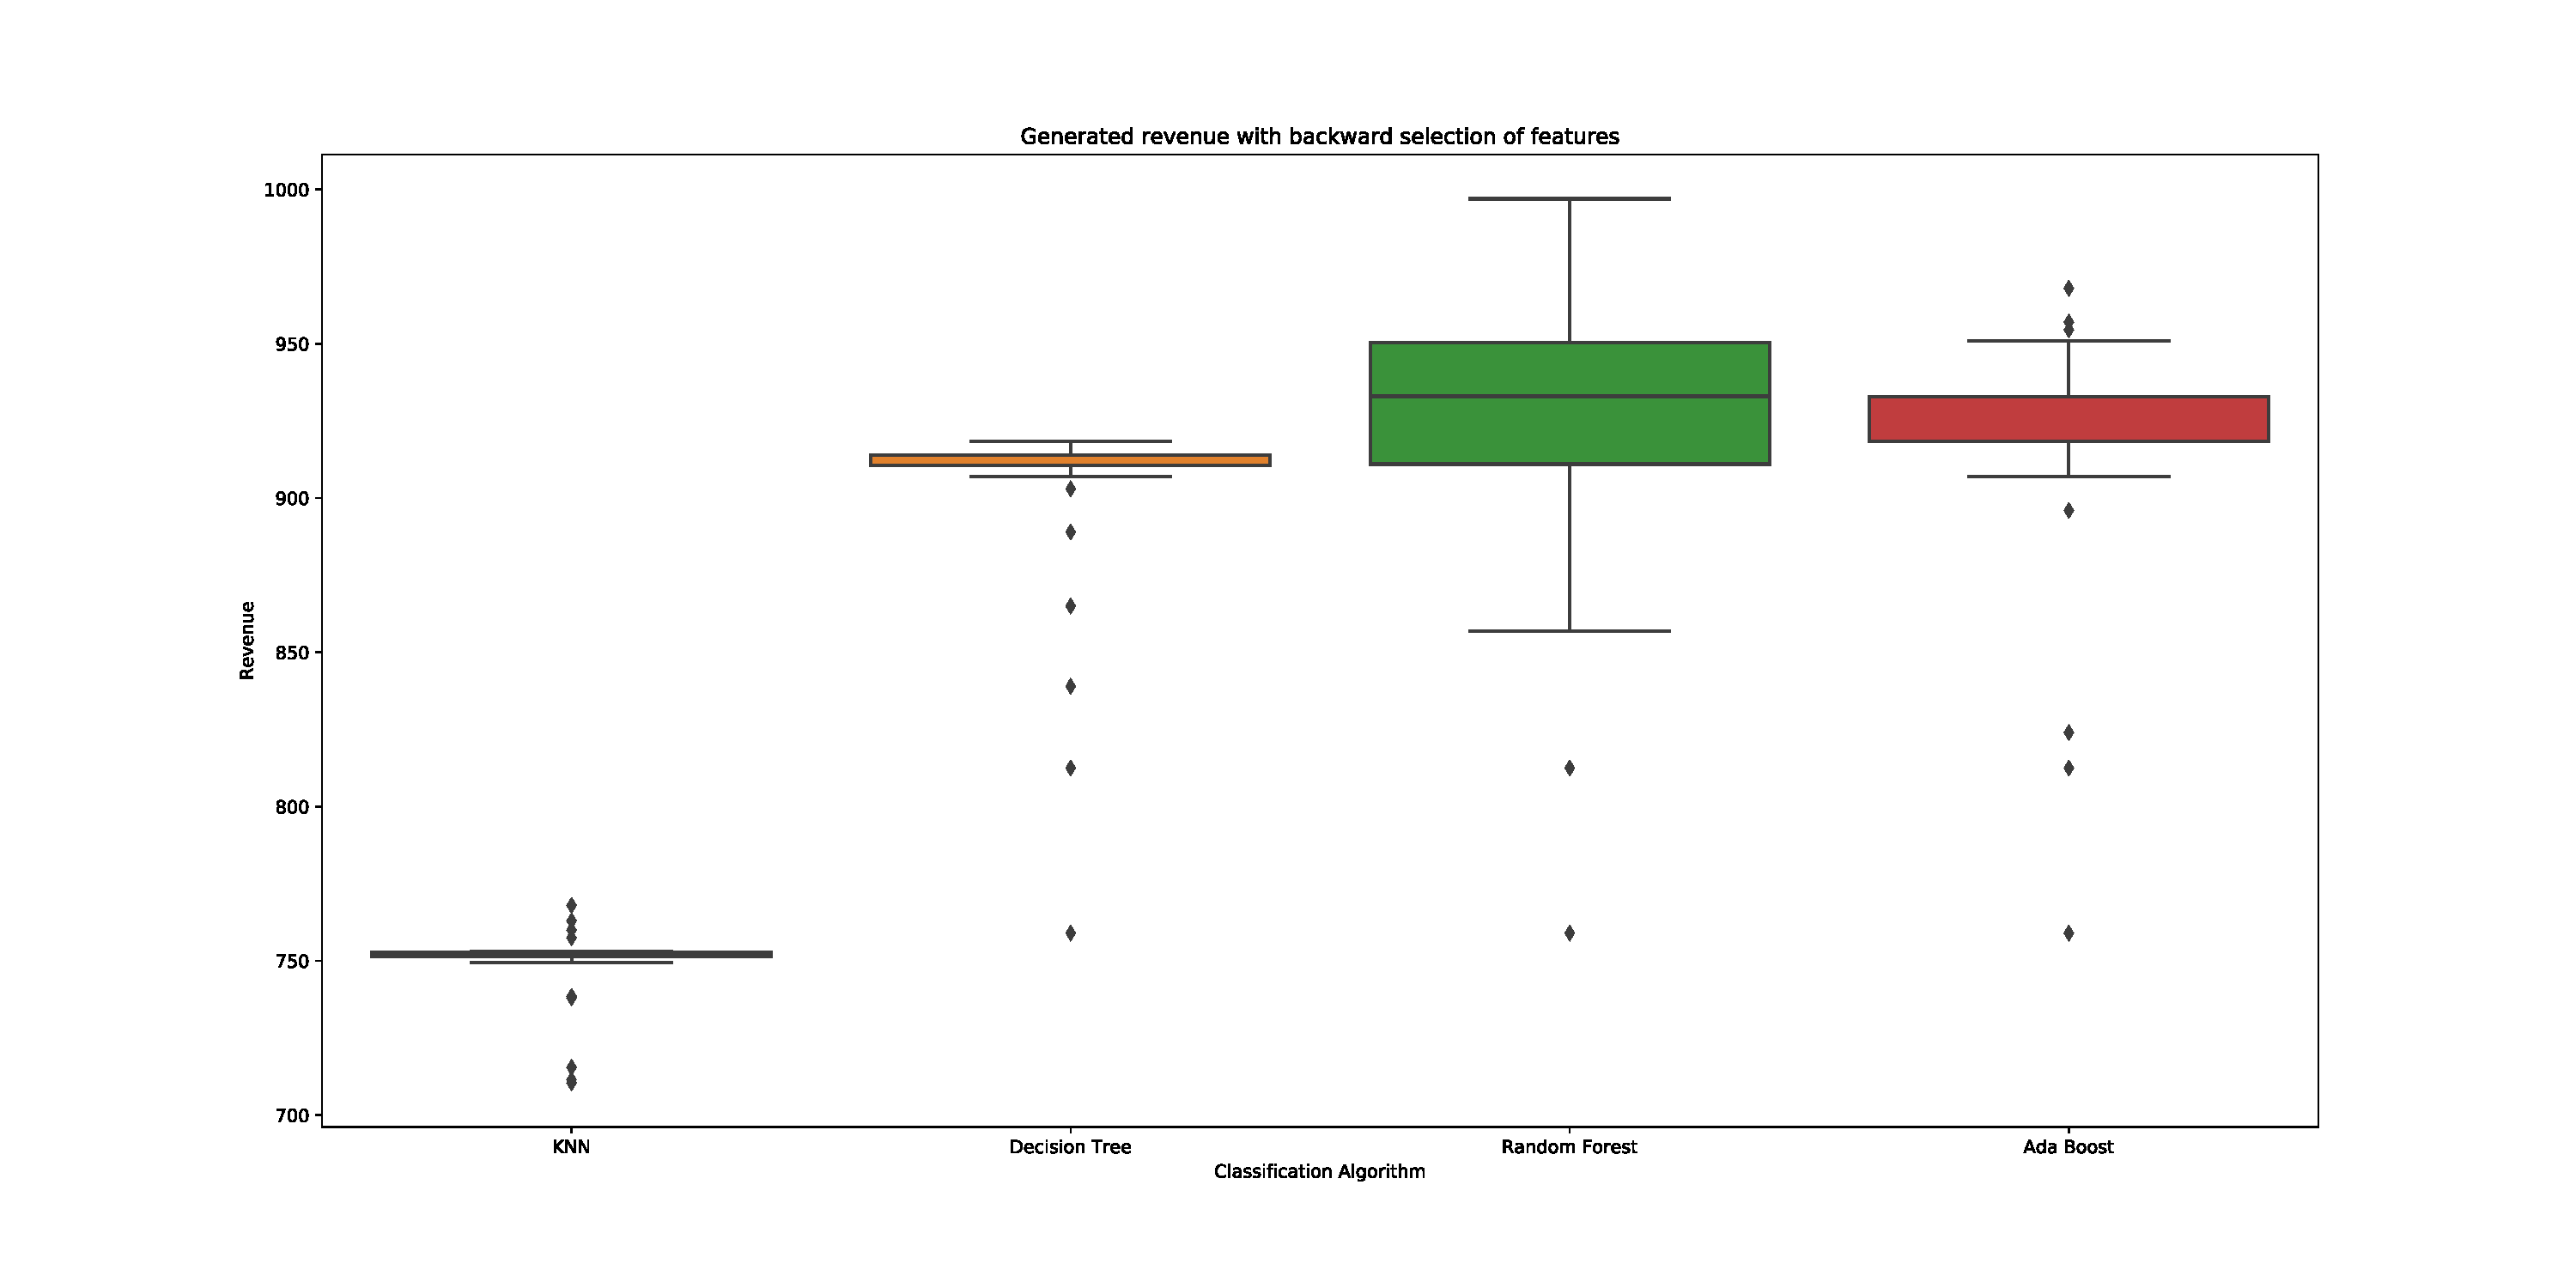
\includegraphics[scale=0.3]{pdf/backward.pdf}
%  \caption{Verteilung der Zielvariable  target90 }
%  \label{fig:backward}
%\end{figure}


\begin{table}[]
\centering
%\begin{tabular}{c c c c c c l}
\begin{tabular*}{\textwidth}{c @{\extracolsep{\fill}} lllllll}
\toprule
\textbf{Rev.} & \textbf{CART} & \textbf{Iter.} & \textbf{Rev.} & \textbf{RF} & \textbf{Rev.} &\textbf{AdaBoost} \\
\midrule
903.0 & w9 & 1 & 857.0 & numberitems & 918.5 & books\\
910.5 & nobooks & 2 & 962.5 & paymenttype0 & 918.5 & paymenttype1\\
910.5 & paymenttype0  & 3 & 931.5 & books & 918.5 & paymenttype1\\
910.5 & paymenttype1 & 4 & 980.0 & paymenttype2 & 918.5 & paymenttype3\\
910.5 & paymenttype2 & 5 & 997.0 & model2 & 918.5 & model1\\
910.5 & paymenttype3 & 6 & 958.0 & advertising & 918.5 & model2\\
910.5 & model1 & 7 & 932.0 & model3 & 918.5 & salutation0 \\
910.5 & model2 & 8 & 951.0 & salutation1 & 918.5 & salutation1\\
910.5 & model3 & 9 & 940.5 & model1 & 918.5 & advertising\\
910.5 & salutation0  & 10 & 928.5 & entry & 918.5 & entry\\
910.5 & salutation1 & 11 & 899.5 & deliverydiff & 918.5 & w4\\
910.5 & salutation2 & 12 & 940.0 & accountdur & 918.5 & w8\\
910.5 & voucher & 13 & 944.5 & w10 & 918.5 & itemseff\\
910.5 & advertising & 14 & 934.0 & voucher & 918.5 & deliverydiff\\
910.5 & numberitems & 15 & 964.0 & w1 & 916.5 & nobooks\\
911.0 & books & 16 & 910.5 & nobooks & 936.0 & case\\
911.0 & entry & 17 & 949.0 & salutation2 & 937.5 & w5\\
911.0 & cancel & 18 & 976.5 & paymenttype3 & 922.0 & w1\\
911.0 & used & 19 & 921.5 & salutation0  & 928.5 & deliverytype\\
914.0 & weight & 20 & 962.5 & w0 & 957.0 & w10\\
914.0 & w0 & 21 & 964.0 & w4 & 957.0 & paymenttype0 \\
914.0 & w6 & 22 & 914.0 & itemseff & 941.0 & w6\\
914.0 & w3 & 23 & 931.5 & shippingcosts & 939.0 & w9\\
918.5 & w4 & 24 & 912.5 & used & 933.0 & used\\
918.5 & w8 & 25 & 935.0 & w2 & 926.5 & w2\\
918.5 & deliverydiff & 26 & 903.5 & w6 & 907.0 & numberitems\\
918.5 & w7 & 27 & 915.0 & paymenttype1 & 932.5 & voucher\\
918.5 & accountdur & 28 & 913.5 & w8 & 954.5 & w0\\
914.0 & case & 29 & 942.0 & cancel & 951.0 & salutation2\\
917.5 & w5 & 30 & 947.5 & w9 & 968.0 & shippingcosts\\
913.0 & w2 & 31 & 934.0 & w7 & 921.5 & model3\\
907.0 & shippingcosts & 32 & 960.0 & w5 & 920.0 & cancel\\
889.0 & w1 & 33 & 909.5 & case & 908.0 & w7\\
839.0 & itemseff & 34 & 899.5 & w3 & 896.0 & w3\\
865.0 & w10 & 35 & 865.0 & weight & 824.0 & weight\\
812.5 & deliverytype & 36 & 812.5 & deliverytype & 812.5 & accountdur\\
759.0 & remi & 37 & 759.0 & remi & 759.0 & remi\\
759.0 & newsletter & 38 & 759.0 & newsletter & 759.0 & newsletter\\
\bottomrule
\end{tabular*}
\caption{Ergebnisse Backward Feature Elimination}
\label{table: Backward}
\end{table}
\FloatBarrier
 
 
\subsection{Evaluation des besten Klassifikators}

Anhand der Backward Feature Elimination ist das Modell ermittelt worden, welches den höchsten Umsatz auf den Testdaten generiert. Das beste Ergebnis erzeugt ein Random-Forest-Klassifikator mit 10 Entscheidungsbäumen, welche auf eine maximale Tiefe von 5 beschränkt worden sind. Dieser ist mit 33 Merkmalen auf einer artifiziell vergrößerten Trainingsdatenbasis trainiert worden und erreicht einen Umsatz von 997 \euro{}. Der Basisumsatz von 674.5 \euro{} wird ohne Klassifikator, durch das Senden von Gutscheinen an alle Kunden, erreicht. Dieser Umsatz ist um 47.81 \% übertroffen worden. Das Modell nutzt einen relativ großen Merkmalsanteil der gegebenen Datenmatrix. Einschränkend muss dazu erwähnt werden, dass bei der Backward Feature Elimination kein Strafterm für die Anzahl der Merkmale eingeflossen ist. Es gibt in Tabelle \ref{table: Backward} ein Modell, welches bereits mit sieben Merkmalen einen Umsatz von 960 \euro{} erzielt. Einfachere Modell sind prinzipiell zu bevorzugen. Die Aufgabenstellung gibt als Zielsetzung die reine Umsatzmaximierung vor. Eine Restriktion bezüglich der Komplexität des Modells gibt es nicht. Daher wird ausschließlich das umsatzstärkste Modell ausführlich evaluiert.\\

\FloatBarrier
\begin{figure}[!htbp]
\begin{center}
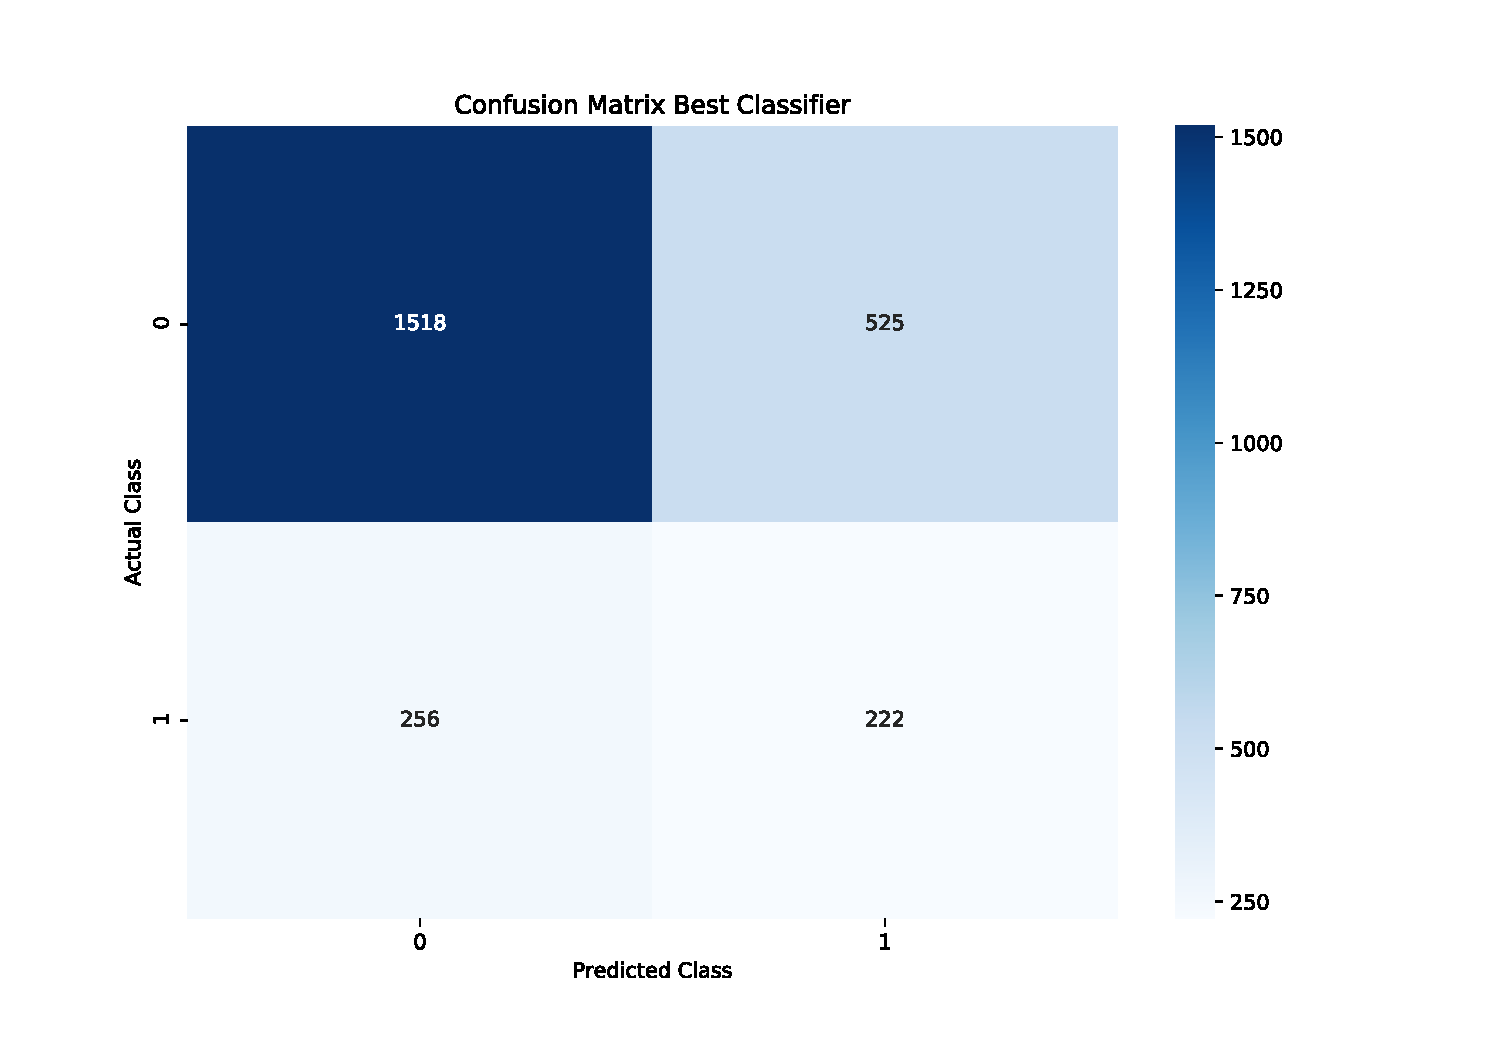
\includegraphics[scale=0.5]{pdf/ConfbestClassifier.pdf}
\end{center}
\caption{Konfusionsmatrix des besten Klassifikators}
\label{fig:confusionFinal}
\end{figure}
\FloatBarrier

In Abbildung \ref{fig:confusionFinal} ist die Konfusionsmatrix des besten Klassifikators abgebildet. Insgesamt sind die Klassen der 2521 Einträge der gegeben Testdaten vorhergesagt worden. Der Testdatensatz besteht aus 2043 Einträgen der Klasse 0 (keine Wiederkäufer) und aus 478 Wiederkäufern (Klasse 1). Von allen Nichtwiederkäufern findet der Klassifikator 74 \% wieder (Recall). Die Präzision der Vorhersage beträgt 86 \% (Precision). Daraus ergibt sich ein F1-Score von 0.8 für Klasse 0. Deutlich schlechter sind die Vorhersagen für die unterrepräsentierte Klasse 1. Diese wird in nur 30 \% der Fälle (Precision) richtig ermittelt. Darüber hinaus wird weniger als die Hälfte der Wiederkäufer wiedergefunden (Recall = 46 \%). Ein deutlich schlechterer F1-Score von 0.36 resultiert unmittelbar, da dieses Maß das harmonische Mittel aus Precision und Recall bildet.\\ 

Generell sollten sich möglichst viele Werte auf der Hauptdiagonalen befinden. Insgesamt werden rund 70 \% der Label richtig vorhergesagt. Der Klassifikator liefert im Hinblick auf die Umsatzsteigerung zufriedenstellende Ergebnisse. Dennoch wird deutlich, dass die Hauptproblematik das Wiederfinden der Kunden ist, welche nach 90 Tagen eine Folgebestellung ausführen. Die Visualisierung von zwei Hauptkomponenten hat starke Überlappungen der Klassengebiete bezüglich der kardinalskalierten Merkmale gezeigt. Auch im Data Understanding Teil ist bereits darauf hingewiesen worden, dass nur wenige kategoriale Merkmale, wie beispielsweise der Newsletter, bezüglich der Klasse diskriminieren. Diese Beobachtung ist mit der Backward Feature Elimination bestätigt worden. Denn selbst das Löschen von über 30 Merkmalen hat keine drastischen Auswirkungen auf die Klassifikatoren gehabt. Aus der Sicht des Business Understandings ist daher darauf zu verweisen, dass das Unternehmen die Ermittlung weiterer, aussagekräftigerer Kennzahlen in Betracht ziehen sollte.   


\begin{table}[]
\centering
%\begin{tabular}{c c c c c c l}
\begin{tabular*}{\textwidth}{c @{\extracolsep{\fill}} lllll}
\toprule
\textbf{Klasse} & \textbf{Precision} & \textbf{Recall} & \textbf{F1-Score} & \textbf{Support}\\
\midrule
0 & 0.86 & 0.74 & 0.80 & 2043\\
1 & 0.30 & 0.46 & 0.36 & 478\\
\midrule
\textbf{Accuracy} &  &  & 0.69 & 2521\\
\bottomrule
\end{tabular*}
\caption{Evaluationsmetriken bester Klassifikator}
\label{table: Backward}
\end{table}
\FloatBarrier

\chapter{Zusammenfassung}

In dieser Projektarbeit ist die Aufgabenstellung des Data Mining Cups 2010 mithilfe eines Teildatensatzes der Originaldaten bearbeitet worden. Das Hauptziel der Aufgabenstellung ist Entwicklung eines binären Klassifikators gewesen, welcher auf einem Testdatensatz einen möglichst hohen Umsatz generieren sollte. Zur Berechnung der Höhe des Umsatzes ist eine Kostenmatrix zur Verfügung gestellt worden.\\ 

Der einfache Ansatz jedem Kunden einen Gutschein in Höhe von 5 \euro{} zu senden, ergibt einen Basisumsatz von 674.5 \euro{}. Dieser Basisumsatz ist durch die intelligente Vergabe von Gutscheine um 47.81 \% auf 997 \euro{} gesteigert worden. Die Ergebnisse sind mithilfe von Methoden des Data Minings und Maschinellen Lernes erreicht worden. Das Vorgehen ist mithilfe des CRISP-DM Modells strukturiert worden.\\ 

In der Business Understanding Phase ist die Aufgabenstellung genau untersucht worden. Die Data Understanding Phase hat mit Methoden der deskriptiven Statistik und einer explorativen Untersuchung des Datensatze den Grundstein für die nachgeschalteten Phasen geliefert. Bei der Datenvorverarbeitung (Data Preparation) ist der Datensatz gezielt durch Feature Engineering und Merkmalstransformationen modifiziert worden, um erfolgsversprechende Modelle zu liefern.\\

Als erste Richtlinie für die Höhe des möglichen Umsatzes hat der k-Nearest-Neighbor-Algorithmus gedient. Aufgrund des heterogenen Datensatzes, bezüglich der Merkmalsskalierung ist anschließend die Wahl auf baumartige Klassifikationsalgorithmen gefallen. Neben klassischen Methoden, wie einfachen Klassifikationsbäumen, sind Ensemble Methoden verwendet worden. Als Vertreter eines Bagging-Klassifikators ist der Random-Forest-Klassifikator gewählt worden. Unter den Boosting Ansätzen ist sich für den AdaBoost Algorithmus mit Entscheidungsbäumen entschieden worden.\\

Mithilfe einer Backward Feature Elimination ist der Einfluss der Merkmalsanzahl auf die Klassifikationsgüte ermittelt worden. Dabei ist gezeigt worden, dass selbst mit einer geringen Anzahl von vielversprechenden Merkmalen gute Ergbenisse erzielt werden können. Das umsatzstärkste Modell hat ein Random-Forest-Klassifikator mit 33 Merkmalen und 10 Klassifikationsbäumen mit einer maximalen Tiefe von 5 geliefert. Dieses Modell ist im letzten Schritt der Ausarbeitung ausführlich evaluiert worden. 




